% Options for packages loaded elsewhere
\PassOptionsToPackage{unicode}{hyperref}
\PassOptionsToPackage{hyphens}{url}
%
\documentclass[
]{article}
\usepackage{amsmath,amssymb}
\usepackage{iftex}
\ifPDFTeX
  \usepackage[T1]{fontenc}
  \usepackage[utf8]{inputenc}
  \usepackage{textcomp} % provide euro and other symbols
\else % if luatex or xetex
  \usepackage{unicode-math} % this also loads fontspec
  \defaultfontfeatures{Scale=MatchLowercase}
  \defaultfontfeatures[\rmfamily]{Ligatures=TeX,Scale=1}
\fi
\usepackage{lmodern}
\ifPDFTeX\else
  % xetex/luatex font selection
\fi
% Use upquote if available, for straight quotes in verbatim environments
\IfFileExists{upquote.sty}{\usepackage{upquote}}{}
\IfFileExists{microtype.sty}{% use microtype if available
  \usepackage[]{microtype}
  \UseMicrotypeSet[protrusion]{basicmath} % disable protrusion for tt fonts
}{}
\makeatletter
\@ifundefined{KOMAClassName}{% if non-KOMA class
  \IfFileExists{parskip.sty}{%
    \usepackage{parskip}
  }{% else
    \setlength{\parindent}{0pt}
    \setlength{\parskip}{6pt plus 2pt minus 1pt}}
}{% if KOMA class
  \KOMAoptions{parskip=half}}
\makeatother
\usepackage{xcolor}
\usepackage[margin=1in]{geometry}
\usepackage{color}
\usepackage{fancyvrb}
\newcommand{\VerbBar}{|}
\newcommand{\VERB}{\Verb[commandchars=\\\{\}]}
\DefineVerbatimEnvironment{Highlighting}{Verbatim}{commandchars=\\\{\}}
% Add ',fontsize=\small' for more characters per line
\usepackage{framed}
\definecolor{shadecolor}{RGB}{248,248,248}
\newenvironment{Shaded}{\begin{snugshade}}{\end{snugshade}}
\newcommand{\AlertTok}[1]{\textcolor[rgb]{0.94,0.16,0.16}{#1}}
\newcommand{\AnnotationTok}[1]{\textcolor[rgb]{0.56,0.35,0.01}{\textbf{\textit{#1}}}}
\newcommand{\AttributeTok}[1]{\textcolor[rgb]{0.13,0.29,0.53}{#1}}
\newcommand{\BaseNTok}[1]{\textcolor[rgb]{0.00,0.00,0.81}{#1}}
\newcommand{\BuiltInTok}[1]{#1}
\newcommand{\CharTok}[1]{\textcolor[rgb]{0.31,0.60,0.02}{#1}}
\newcommand{\CommentTok}[1]{\textcolor[rgb]{0.56,0.35,0.01}{\textit{#1}}}
\newcommand{\CommentVarTok}[1]{\textcolor[rgb]{0.56,0.35,0.01}{\textbf{\textit{#1}}}}
\newcommand{\ConstantTok}[1]{\textcolor[rgb]{0.56,0.35,0.01}{#1}}
\newcommand{\ControlFlowTok}[1]{\textcolor[rgb]{0.13,0.29,0.53}{\textbf{#1}}}
\newcommand{\DataTypeTok}[1]{\textcolor[rgb]{0.13,0.29,0.53}{#1}}
\newcommand{\DecValTok}[1]{\textcolor[rgb]{0.00,0.00,0.81}{#1}}
\newcommand{\DocumentationTok}[1]{\textcolor[rgb]{0.56,0.35,0.01}{\textbf{\textit{#1}}}}
\newcommand{\ErrorTok}[1]{\textcolor[rgb]{0.64,0.00,0.00}{\textbf{#1}}}
\newcommand{\ExtensionTok}[1]{#1}
\newcommand{\FloatTok}[1]{\textcolor[rgb]{0.00,0.00,0.81}{#1}}
\newcommand{\FunctionTok}[1]{\textcolor[rgb]{0.13,0.29,0.53}{\textbf{#1}}}
\newcommand{\ImportTok}[1]{#1}
\newcommand{\InformationTok}[1]{\textcolor[rgb]{0.56,0.35,0.01}{\textbf{\textit{#1}}}}
\newcommand{\KeywordTok}[1]{\textcolor[rgb]{0.13,0.29,0.53}{\textbf{#1}}}
\newcommand{\NormalTok}[1]{#1}
\newcommand{\OperatorTok}[1]{\textcolor[rgb]{0.81,0.36,0.00}{\textbf{#1}}}
\newcommand{\OtherTok}[1]{\textcolor[rgb]{0.56,0.35,0.01}{#1}}
\newcommand{\PreprocessorTok}[1]{\textcolor[rgb]{0.56,0.35,0.01}{\textit{#1}}}
\newcommand{\RegionMarkerTok}[1]{#1}
\newcommand{\SpecialCharTok}[1]{\textcolor[rgb]{0.81,0.36,0.00}{\textbf{#1}}}
\newcommand{\SpecialStringTok}[1]{\textcolor[rgb]{0.31,0.60,0.02}{#1}}
\newcommand{\StringTok}[1]{\textcolor[rgb]{0.31,0.60,0.02}{#1}}
\newcommand{\VariableTok}[1]{\textcolor[rgb]{0.00,0.00,0.00}{#1}}
\newcommand{\VerbatimStringTok}[1]{\textcolor[rgb]{0.31,0.60,0.02}{#1}}
\newcommand{\WarningTok}[1]{\textcolor[rgb]{0.56,0.35,0.01}{\textbf{\textit{#1}}}}
\usepackage{graphicx}
\makeatletter
\def\maxwidth{\ifdim\Gin@nat@width>\linewidth\linewidth\else\Gin@nat@width\fi}
\def\maxheight{\ifdim\Gin@nat@height>\textheight\textheight\else\Gin@nat@height\fi}
\makeatother
% Scale images if necessary, so that they will not overflow the page
% margins by default, and it is still possible to overwrite the defaults
% using explicit options in \includegraphics[width, height, ...]{}
\setkeys{Gin}{width=\maxwidth,height=\maxheight,keepaspectratio}
% Set default figure placement to htbp
\makeatletter
\def\fps@figure{htbp}
\makeatother
\setlength{\emergencystretch}{3em} % prevent overfull lines
\providecommand{\tightlist}{%
  \setlength{\itemsep}{0pt}\setlength{\parskip}{0pt}}
\setcounter{secnumdepth}{-\maxdimen} % remove section numbering
\ifLuaTeX
  \usepackage{selnolig}  % disable illegal ligatures
\fi
\usepackage{bookmark}
\IfFileExists{xurl.sty}{\usepackage{xurl}}{} % add URL line breaks if available
\urlstyle{same}
\hypersetup{
  pdftitle={Cyclistics},
  pdfauthor={marely},
  hidelinks,
  pdfcreator={LaTeX via pandoc}}

\title{Cyclistics}
\author{marely}
\date{18-01-2024}

\begin{document}
\maketitle

\section{Preparación de Datos}\label{preparaciuxf3n-de-datos}

\hfill\break
\textbf{Paso 1.} Instalación y carga del paquete \texttt{Tidyverse}

\begin{Shaded}
\begin{Highlighting}[]
\ControlFlowTok{if}\NormalTok{ (}\SpecialCharTok{!}\FunctionTok{requireNamespace}\NormalTok{(}\StringTok{"tidyverse"}\NormalTok{, }\AttributeTok{quietly =} \ConstantTok{TRUE}\NormalTok{)) }
  \FunctionTok{install.packages}\NormalTok{(}\StringTok{"tidyverse"}\NormalTok{) }
\FunctionTok{library}\NormalTok{(tidyverse) }
\end{Highlighting}
\end{Shaded}

\begin{verbatim}
## -- Attaching core tidyverse packages ------------------------ tidyverse 2.0.0 --
## v dplyr     1.1.4     v readr     2.1.5
## v forcats   1.0.0     v stringr   1.5.1
## v ggplot2   3.5.1     v tibble    3.2.1
## v lubridate 1.9.4     v tidyr     1.3.1
## v purrr     1.0.2     
## -- Conflicts ------------------------------------------ tidyverse_conflicts() --
## x dplyr::filter() masks stats::filter()
## x dplyr::lag()    masks stats::lag()
## i Use the conflicted package (<http://conflicted.r-lib.org/>) to force all conflicts to become errors
\end{verbatim}

\hfill\break
\textbf{Paso 2.} Función para construir rutas.

\begin{Shaded}
\begin{Highlighting}[]
\NormalTok{construir\_ruta }\OtherTok{\textless{}{-}} \ControlFlowTok{function}\NormalTok{(...)\{}
  \FunctionTok{return}\NormalTok{(}\FunctionTok{file.path}\NormalTok{(}\FunctionTok{getwd}\NormalTok{(), ...))}
\NormalTok{\} }
\end{Highlighting}
\end{Shaded}

\hfill\break
\textbf{Paso 3.} Obtener las rutas de datos y datos de origen
(data-meses)

\begin{Shaded}
\begin{Highlighting}[]
\NormalTok{ruta\_datos }\OtherTok{\textless{}{-}} \FunctionTok{construir\_ruta}\NormalTok{(}\StringTok{"data"}\NormalTok{) }
\NormalTok{ruta\_datos\_de\_origen }\OtherTok{\textless{}{-}} \FunctionTok{construir\_ruta}\NormalTok{(}\StringTok{"data"}\NormalTok{, }\StringTok{"data{-}meses"}\NormalTok{)}
\end{Highlighting}
\end{Shaded}

\hfill\break
\textbf{Paso 4.} Cargar y mostrar la lista de archivos csv
correspondiente a los datos mensuales del proyecto.

\begin{Shaded}
\begin{Highlighting}[]
\NormalTok{archivos\_csv }\OtherTok{\textless{}{-}} \FunctionTok{list.files}\NormalTok{(}\AttributeTok{path =}\NormalTok{ ruta\_datos\_de\_origen, }\AttributeTok{pattern =} \StringTok{"}\SpecialCharTok{\textbackslash{}\textbackslash{}}\StringTok{.csv$"}\NormalTok{, }\AttributeTok{full.names =} \ConstantTok{FALSE}\NormalTok{, }\AttributeTok{recursive =} \ConstantTok{TRUE}\NormalTok{)}
\FunctionTok{print}\NormalTok{(archivos\_csv)}
\end{Highlighting}
\end{Shaded}

\begin{verbatim}
##  [1] "202401-divvy-tripdata.csv" "202402-divvy-tripdata.csv"
##  [3] "202403-divvy-tripdata.csv" "202404-divvy-tripdata.csv"
##  [5] "202405-divvy-tripdata.csv" "202406-divvy-tripdata.csv"
##  [7] "202407-divvy-tripdata.csv" "202408-divvy-tripdata.csv"
##  [9] "202409-divvy-tripdata.csv" "202410-divvy-tripdata.csv"
## [11] "202411-divvy-tripdata.csv" "202412-divvy-tripdata.csv"
\end{verbatim}

\hfill\break
\textbf{Paso 5.} Iterar sobre los archivos csv para visualizar las
columnas.

\begin{Shaded}
\begin{Highlighting}[]
\ControlFlowTok{for}\NormalTok{ (archivo }\ControlFlowTok{in}\NormalTok{ archivos\_csv) \{ }
  \FunctionTok{tryCatch}\NormalTok{(\{}
\NormalTok{    datos }\OtherTok{\textless{}{-}} \FunctionTok{read.csv}\NormalTok{(}\FunctionTok{file.path}\NormalTok{(ruta\_datos\_de\_origen, archivo)) }
    \FunctionTok{print}\NormalTok{(}\FunctionTok{paste}\NormalTok{(}\StringTok{\textquotesingle{}NOMBRE ARCHIVO: \textquotesingle{}}\NormalTok{, archivo))}
    \FunctionTok{print}\NormalTok{(}\FunctionTok{colnames}\NormalTok{(datos))}
    \FunctionTok{str}\NormalTok{(datos)}
    \FunctionTok{cat}\NormalTok{(}\StringTok{"}\SpecialCharTok{\textbackslash{}n}\StringTok{"}\NormalTok{)}
\NormalTok{  \}, }\AttributeTok{error =} \ControlFlowTok{function}\NormalTok{(e) \{}
    \FunctionTok{message}\NormalTok{(}\StringTok{"Error leyendo archivo: "}\NormalTok{, archivo, }\StringTok{"}\SpecialCharTok{\textbackslash{}n}\StringTok{"}\NormalTok{, e)}
\NormalTok{  \})}
\NormalTok{\}}
\end{Highlighting}
\end{Shaded}

\begin{verbatim}
## [1] "NOMBRE ARCHIVO:  202401-divvy-tripdata.csv"
##  [1] "ride_id"            "rideable_type"      "started_at"        
##  [4] "ended_at"           "start_station_name" "start_station_id"  
##  [7] "end_station_name"   "end_station_id"     "start_lat"         
## [10] "start_lng"          "end_lat"            "end_lng"           
## [13] "member_casual"     
## 'data.frame':    144873 obs. of  13 variables:
##  $ ride_id           : chr  "C1D650626C8C899A" "EECD38BDB25BFCB0" "F4A9CE78061F17F7" "0A0D9E15EE50B171" ...
##  $ rideable_type     : chr  "electric_bike" "electric_bike" "electric_bike" "classic_bike" ...
##  $ started_at        : chr  "2024-01-12 15:30:27" "2024-01-08 15:45:46" "2024-01-27 12:27:19" "2024-01-29 16:26:17" ...
##  $ ended_at          : chr  "2024-01-12 15:37:59" "2024-01-08 15:52:59" "2024-01-27 12:35:19" "2024-01-29 16:56:06" ...
##  $ start_station_name: chr  "Wells St & Elm St" "Wells St & Elm St" "Wells St & Elm St" "Wells St & Randolph St" ...
##  $ start_station_id  : chr  "KA1504000135" "KA1504000135" "KA1504000135" "TA1305000030" ...
##  $ end_station_name  : chr  "Kingsbury St & Kinzie St" "Kingsbury St & Kinzie St" "Kingsbury St & Kinzie St" "Larrabee St & Webster Ave" ...
##  $ end_station_id    : chr  "KA1503000043" "KA1503000043" "KA1503000043" "13193" ...
##  $ start_lat         : num  41.9 41.9 41.9 41.9 41.9 ...
##  $ start_lng         : num  -87.6 -87.6 -87.6 -87.6 -87.7 ...
##  $ end_lat           : num  41.9 41.9 41.9 41.9 41.9 ...
##  $ end_lng           : num  -87.6 -87.6 -87.6 -87.6 -87.6 ...
##  $ member_casual     : chr  "member" "member" "member" "member" ...
## 
## [1] "NOMBRE ARCHIVO:  202402-divvy-tripdata.csv"
##  [1] "ride_id"            "rideable_type"      "started_at"        
##  [4] "ended_at"           "start_station_name" "start_station_id"  
##  [7] "end_station_name"   "end_station_id"     "start_lat"         
## [10] "start_lng"          "end_lat"            "end_lng"           
## [13] "member_casual"     
## 'data.frame':    223164 obs. of  13 variables:
##  $ ride_id           : chr  "FCB05EB1758F85E8" "7FB986AD5D3DE9D6" "40CA13E15B5B470D" "D47A1660919E8861" ...
##  $ rideable_type     : chr  "classic_bike" "classic_bike" "electric_bike" "classic_bike" ...
##  $ started_at        : chr  "2024-02-03 14:14:18" "2024-02-05 21:10:06" "2024-02-05 15:10:44" "2024-02-15 12:40:34" ...
##  $ ended_at          : chr  "2024-02-03 14:21:00" "2024-02-05 21:15:44" "2024-02-05 15:12:32" "2024-02-15 12:44:24" ...
##  $ start_station_name: chr  "Clark St & Newport St" "Michigan Ave & Washington St" "Leavitt St & Armitage Ave" "Southport Ave & Waveland Ave" ...
##  $ start_station_id  : chr  "632" "13001" "TA1309000029" "13235" ...
##  $ end_station_name  : chr  "Southport Ave & Waveland Ave" "Wabash Ave & Grand Ave" "Milwaukee Ave & Wabansia Ave" "Southport Ave & Belmont Ave" ...
##  $ end_station_id    : chr  "13235" "TA1307000117" "13243" "13229" ...
##  $ start_lat         : num  41.9 41.9 41.9 41.9 41.8 ...
##  $ start_lng         : num  -87.7 -87.6 -87.7 -87.7 -87.6 ...
##  $ end_lat           : num  41.9 41.9 41.9 41.9 41.8 ...
##  $ end_lng           : num  -87.7 -87.6 -87.7 -87.7 -87.6 ...
##  $ member_casual     : chr  "member" "member" "member" "member" ...
## 
## [1] "NOMBRE ARCHIVO:  202403-divvy-tripdata.csv"
##  [1] "ride_id"            "rideable_type"      "started_at"        
##  [4] "ended_at"           "start_station_name" "start_station_id"  
##  [7] "end_station_name"   "end_station_id"     "start_lat"         
## [10] "start_lng"          "end_lat"            "end_lng"           
## [13] "member_casual"     
## 'data.frame':    301687 obs. of  13 variables:
##  $ ride_id           : chr  "64FBE3BAED5F29E6" "9991629435C5E20E" "E5C9FECD5B71BEBD" "4CEA3EC8906DAEA8" ...
##  $ rideable_type     : chr  "electric_bike" "electric_bike" "electric_bike" "electric_bike" ...
##  $ started_at        : chr  "2024-03-05 18:33:11" "2024-03-06 17:15:14" "2024-03-06 17:16:36" "2024-03-03 22:55:54" ...
##  $ ended_at          : chr  "2024-03-05 18:51:48" "2024-03-06 17:16:04" "2024-03-06 17:19:28" "2024-03-03 22:58:08" ...
##  $ start_station_name: chr  "" "" "" "" ...
##  $ start_station_id  : chr  "" "" "" "" ...
##  $ end_station_name  : chr  "" "" "" "" ...
##  $ end_station_id    : chr  "" "" "" "" ...
##  $ start_lat         : num  41.9 41.9 41.9 41.9 41.9 ...
##  $ start_lng         : num  -87.7 -87.6 -87.6 -87.6 -87.7 ...
##  $ end_lat           : num  42 41.9 41.9 41.9 41.9 ...
##  $ end_lng           : num  -87.7 -87.6 -87.6 -87.6 -87.7 ...
##  $ member_casual     : chr  "member" "member" "member" "member" ...
## 
## [1] "NOMBRE ARCHIVO:  202404-divvy-tripdata.csv"
##  [1] "ride_id"            "rideable_type"      "started_at"        
##  [4] "ended_at"           "start_station_name" "start_station_id"  
##  [7] "end_station_name"   "end_station_id"     "start_lat"         
## [10] "start_lng"          "end_lat"            "end_lng"           
## [13] "member_casual"     
## 'data.frame':    415025 obs. of  13 variables:
##  $ ride_id           : chr  "743252713F32516B" "BE90D33D2240C614" "D47BBDDE7C40DD61" "6684E760BF9EA9B5" ...
##  $ rideable_type     : chr  "classic_bike" "electric_bike" "classic_bike" "classic_bike" ...
##  $ started_at        : chr  "2024-04-22 19:08:21" "2024-04-11 06:19:24" "2024-04-20 11:13:13" "2024-04-04 18:39:20" ...
##  $ ended_at          : chr  "2024-04-22 19:12:56" "2024-04-11 06:22:21" "2024-04-20 11:29:31" "2024-04-04 18:43:06" ...
##  $ start_station_name: chr  "Aberdeen St & Jackson Blvd" "Aberdeen St & Jackson Blvd" "Sheridan Rd & Montrose Ave" "Aberdeen St & Jackson Blvd" ...
##  $ start_station_id  : chr  "13157" "13157" "TA1307000107" "13157" ...
##  $ end_station_name  : chr  "Desplaines St & Jackson Blvd" "Desplaines St & Jackson Blvd" "Ashland Ave & Belle Plaine Ave" "Desplaines St & Jackson Blvd" ...
##  $ end_station_id    : chr  "15539" "15539" "13249" "15539" ...
##  $ start_lat         : num  41.9 41.9 42 41.9 42 ...
##  $ start_lng         : num  -87.7 -87.7 -87.7 -87.7 -87.7 ...
##  $ end_lat           : num  41.9 41.9 42 41.9 41.9 ...
##  $ end_lng           : num  -87.6 -87.6 -87.7 -87.6 -87.6 ...
##  $ member_casual     : chr  "member" "member" "member" "member" ...
## 
## [1] "NOMBRE ARCHIVO:  202405-divvy-tripdata.csv"
##  [1] "ride_id"            "rideable_type"      "started_at"        
##  [4] "ended_at"           "start_station_name" "start_station_id"  
##  [7] "end_station_name"   "end_station_id"     "start_lat"         
## [10] "start_lng"          "end_lat"            "end_lng"           
## [13] "member_casual"     
## 'data.frame':    609493 obs. of  13 variables:
##  $ ride_id           : chr  "7D9F0CE9EC2A1297" "02EC47687411416F" "101370FB2D3402BE" "E97E396331ED6913" ...
##  $ rideable_type     : chr  "classic_bike" "classic_bike" "classic_bike" "electric_bike" ...
##  $ started_at        : chr  "2024-05-25 15:52:42" "2024-05-14 15:11:51" "2024-05-30 17:46:04" "2024-05-17 20:21:54" ...
##  $ ended_at          : chr  "2024-05-25 16:11:50" "2024-05-14 15:22:00" "2024-05-30 18:09:16" "2024-05-17 20:40:32" ...
##  $ start_station_name: chr  "Streeter Dr & Grand Ave" "Sheridan Rd & Greenleaf Ave" "Streeter Dr & Grand Ave" "Streeter Dr & Grand Ave" ...
##  $ start_station_id  : chr  "13022" "KA1504000159" "13022" "13022" ...
##  $ end_station_name  : chr  "Clark St & Elm St" "Sheridan Rd & Loyola Ave" "Wabash Ave & 9th St" "Sheffield Ave & Wellington Ave" ...
##  $ end_station_id    : chr  "TA1307000039" "RP-009" "TA1309000010" "TA1307000052" ...
##  $ start_lat         : num  41.9 42 41.9 41.9 41.9 ...
##  $ start_lng         : num  -87.6 -87.7 -87.6 -87.6 -87.6 ...
##  $ end_lat           : num  41.9 42 41.9 41.9 41.9 ...
##  $ end_lng           : num  -87.6 -87.7 -87.6 -87.7 -87.6 ...
##  $ member_casual     : chr  "casual" "casual" "member" "member" ...
## 
## [1] "NOMBRE ARCHIVO:  202406-divvy-tripdata.csv"
##  [1] "ride_id"            "rideable_type"      "started_at"        
##  [4] "ended_at"           "start_station_name" "start_station_id"  
##  [7] "end_station_name"   "end_station_id"     "start_lat"         
## [10] "start_lng"          "end_lat"            "end_lng"           
## [13] "member_casual"     
## 'data.frame':    710721 obs. of  13 variables:
##  $ ride_id           : chr  "CDE6023BE6B11D2F" "462B48CD292B6A18" "9CFB6A858D23ABF7" "6365EFEB64231153" ...
##  $ rideable_type     : chr  "electric_bike" "electric_bike" "electric_bike" "electric_bike" ...
##  $ started_at        : chr  "2024-06-11 17:20:06.289" "2024-06-11 17:19:21.567" "2024-06-11 17:25:27.089" "2024-06-11 11:53:50.769" ...
##  $ ended_at          : chr  "2024-06-11 17:21:39.464" "2024-06-11 17:19:36.377" "2024-06-11 17:30:13.035" "2024-06-11 12:08:13.382" ...
##  $ start_station_name: chr  "" "" "" "" ...
##  $ start_station_id  : chr  "" "" "" "" ...
##  $ end_station_name  : chr  "" "" "" "" ...
##  $ end_station_id    : chr  "" "" "" "" ...
##  $ start_lat         : num  41.9 41.9 41.9 41.9 41.9 ...
##  $ start_lng         : num  -87.7 -87.7 -87.7 -87.6 -87.6 ...
##  $ end_lat           : num  41.9 41.9 41.9 41.9 41.9 ...
##  $ end_lng           : num  -87.7 -87.7 -87.7 -87.6 -87.6 ...
##  $ member_casual     : chr  "casual" "casual" "casual" "casual" ...
## 
## [1] "NOMBRE ARCHIVO:  202407-divvy-tripdata.csv"
##  [1] "ride_id"            "rideable_type"      "started_at"        
##  [4] "ended_at"           "start_station_name" "start_station_id"  
##  [7] "end_station_name"   "end_station_id"     "start_lat"         
## [10] "start_lng"          "end_lat"            "end_lng"           
## [13] "member_casual"     
## 'data.frame':    748962 obs. of  13 variables:
##  $ ride_id           : chr  "2658E319B13141F9" "B2176315168A47CE" "C2A9D33DF7EBB422" "8BFEA406DF01D8AD" ...
##  $ rideable_type     : chr  "electric_bike" "electric_bike" "electric_bike" "electric_bike" ...
##  $ started_at        : chr  "2024-07-11 08:15:14.784" "2024-07-11 15:45:07.851" "2024-07-11 08:24:48.192" "2024-07-11 08:46:06.864" ...
##  $ ended_at          : chr  "2024-07-11 08:17:56.335" "2024-07-11 16:06:04.243" "2024-07-11 08:28:05.237" "2024-07-11 09:14:11.664" ...
##  $ start_station_name: chr  "" "" "" "" ...
##  $ start_station_id  : chr  "" "" "" "" ...
##  $ end_station_name  : chr  "" "" "" "" ...
##  $ end_station_id    : chr  "" "" "" "" ...
##  $ start_lat         : num  41.8 41.8 41.8 41.9 42 ...
##  $ start_lng         : num  -87.6 -87.6 -87.6 -87.6 -87.6 ...
##  $ end_lat           : num  41.8 41.8 41.8 41.9 41.9 ...
##  $ end_lng           : num  -87.6 -87.6 -87.6 -87.7 -87.6 ...
##  $ member_casual     : chr  "casual" "casual" "casual" "casual" ...
## 
## [1] "NOMBRE ARCHIVO:  202408-divvy-tripdata.csv"
##  [1] "ride_id"            "rideable_type"      "started_at"        
##  [4] "ended_at"           "start_station_name" "start_station_id"  
##  [7] "end_station_name"   "end_station_id"     "start_lat"         
## [10] "start_lng"          "end_lat"            "end_lng"           
## [13] "member_casual"     
## 'data.frame':    755639 obs. of  13 variables:
##  $ ride_id           : chr  "BAA154388A869E64" "8752245932EFF67A" "44DDF9F57A9A161F" "44AAAF069B0C78C3" ...
##  $ rideable_type     : chr  "classic_bike" "electric_bike" "classic_bike" "electric_bike" ...
##  $ started_at        : chr  "2024-08-02 13:35:14.403" "2024-08-02 15:33:13.965" "2024-08-16 15:44:06.233" "2024-08-19 18:47:11.855" ...
##  $ ended_at          : chr  "2024-08-02 13:48:24.426" "2024-08-02 15:55:23.865" "2024-08-16 15:57:52.109" "2024-08-19 18:56:33.269" ...
##  $ start_station_name: chr  "State St & Randolph St" "Franklin St & Monroe St" "Franklin St & Monroe St" "Clark St & Elm St" ...
##  $ start_station_id  : chr  "TA1305000029" "TA1309000007" "TA1309000007" "TA1307000039" ...
##  $ end_station_name  : chr  "Wabash Ave & 9th St" "Damen Ave & Cortland St" "Clark St & Elm St" "McClurg Ct & Ohio St" ...
##  $ end_station_id    : chr  "TA1309000010" "13133" "TA1307000039" "TA1306000029" ...
##  $ start_lat         : num  41.9 41.9 41.9 41.9 42 ...
##  $ start_lng         : num  -87.6 -87.6 -87.6 -87.6 -87.7 ...
##  $ end_lat           : num  41.9 41.9 41.9 41.9 42 ...
##  $ end_lng           : num  -87.6 -87.7 -87.6 -87.6 -87.7 ...
##  $ member_casual     : chr  "member" "member" "member" "member" ...
## 
## [1] "NOMBRE ARCHIVO:  202409-divvy-tripdata.csv"
##  [1] "ride_id"            "rideable_type"      "started_at"        
##  [4] "ended_at"           "start_station_name" "start_station_id"  
##  [7] "end_station_name"   "end_station_id"     "start_lat"         
## [10] "start_lng"          "end_lat"            "end_lng"           
## [13] "member_casual"     
## 'data.frame':    821276 obs. of  13 variables:
##  $ ride_id           : chr  "31D38723D5A8665A" "67CB39987F4E895B" "DA61204FD26EC681" "06F160D46AF235DD" ...
##  $ rideable_type     : chr  "electric_bike" "electric_bike" "electric_bike" "electric_bike" ...
##  $ started_at        : chr  "2024-09-26 15:30:58.150" "2024-09-26 15:31:32.529" "2024-09-26 15:00:33.012" "2024-09-26 18:19:06.491" ...
##  $ ended_at          : chr  "2024-09-26 15:30:59.437" "2024-09-26 15:53:13.501" "2024-09-26 15:02:25.406" "2024-09-26 18:38:53.515" ...
##  $ start_station_name: chr  "" "" "" "" ...
##  $ start_station_id  : chr  "" "" "" "" ...
##  $ end_station_name  : chr  "" "" "" "" ...
##  $ end_station_id    : chr  "" "" "" "" ...
##  $ start_lat         : num  41.9 41.9 41.9 41.9 41.9 ...
##  $ start_lng         : num  -87.6 -87.6 -87.6 -87.6 -87.7 ...
##  $ end_lat           : num  41.9 41.9 41.9 41.9 41.9 ...
##  $ end_lng           : num  -87.6 -87.6 -87.6 -87.6 -87.6 ...
##  $ member_casual     : chr  "member" "member" "member" "member" ...
## 
## [1] "NOMBRE ARCHIVO:  202410-divvy-tripdata.csv"
##  [1] "ride_id"            "rideable_type"      "started_at"        
##  [4] "ended_at"           "start_station_name" "start_station_id"  
##  [7] "end_station_name"   "end_station_id"     "start_lat"         
## [10] "start_lng"          "end_lat"            "end_lng"           
## [13] "member_casual"     
## 'data.frame':    616281 obs. of  13 variables:
##  $ ride_id           : chr  "4422E707103AA4FF" "19DB722B44CBE82F" "20AE2509FD68C939" "D0F17580AB9515A9" ...
##  $ rideable_type     : chr  "electric_bike" "electric_bike" "electric_bike" "electric_bike" ...
##  $ started_at        : chr  "2024-10-14 03:26:04.083" "2024-10-13 19:33:38.926" "2024-10-13 23:40:48.522" "2024-10-14 02:13:41.602" ...
##  $ ended_at          : chr  "2024-10-14 03:32:56.535" "2024-10-13 19:39:04.490" "2024-10-13 23:48:02.339" "2024-10-14 02:25:40.057" ...
##  $ start_station_name: chr  "" "" "" "" ...
##  $ start_station_id  : chr  "" "" "" "" ...
##  $ end_station_name  : chr  "" "" "" "" ...
##  $ end_station_id    : chr  "" "" "" "" ...
##  $ start_lat         : num  42 42 42 42 42 ...
##  $ start_lng         : num  -87.7 -87.7 -87.7 -87.7 -87.7 ...
##  $ end_lat           : num  42 42 42 42 42 ...
##  $ end_lng           : num  -87.7 -87.7 -87.7 -87.7 -87.7 ...
##  $ member_casual     : chr  "member" "member" "member" "member" ...
## 
## [1] "NOMBRE ARCHIVO:  202411-divvy-tripdata.csv"
##  [1] "ride_id"            "rideable_type"      "started_at"        
##  [4] "ended_at"           "start_station_name" "start_station_id"  
##  [7] "end_station_name"   "end_station_id"     "start_lat"         
## [10] "start_lng"          "end_lat"            "end_lng"           
## [13] "member_casual"     
## 'data.frame':    335075 obs. of  13 variables:
##  $ ride_id           : chr  "578DDD7CE1771FFA" "78B141C50102ABA6" "1E794CF36394E2D7" "E5DD2CAB58D73F98" ...
##  $ rideable_type     : chr  "classic_bike" "classic_bike" "classic_bike" "classic_bike" ...
##  $ started_at        : chr  "2024-11-07 19:21:58.206" "2024-11-22 14:49:00.431" "2024-11-08 09:24:00.238" "2024-11-24 17:51:14.144" ...
##  $ ended_at          : chr  "2024-11-07 19:28:57.301" "2024-11-22 14:56:15.475" "2024-11-08 09:28:33.480" "2024-11-24 18:05:32.574" ...
##  $ start_station_name: chr  "Walsh Park" "Walsh Park" "Walsh Park" "Clark St & Elm St" ...
##  $ start_station_id  : chr  "18067" "18067" "18067" "TA1307000039" ...
##  $ end_station_name  : chr  "Leavitt St & North Ave" "Leavitt St & Armitage Ave" "Damen Ave & Cortland St" "Clark St & Drummond Pl" ...
##  $ end_station_id    : chr  "TA1308000005" "TA1309000029" "13133" "TA1307000142" ...
##  $ start_lat         : num  41.9 41.9 41.9 41.9 41.9 ...
##  $ start_lng         : num  -87.7 -87.7 -87.7 -87.6 -87.6 ...
##  $ end_lat           : num  41.9 41.9 41.9 41.9 41.9 ...
##  $ end_lng           : num  -87.7 -87.7 -87.7 -87.6 -87.6 ...
##  $ member_casual     : chr  "member" "member" "member" "member" ...
## 
## [1] "NOMBRE ARCHIVO:  202412-divvy-tripdata.csv"
##  [1] "ride_id"            "rideable_type"      "started_at"        
##  [4] "ended_at"           "start_station_name" "start_station_id"  
##  [7] "end_station_name"   "end_station_id"     "start_lat"         
## [10] "start_lng"          "end_lat"            "end_lng"           
## [13] "member_casual"     
## 'data.frame':    178372 obs. of  13 variables:
##  $ ride_id           : chr  "6C960DEB4F78854E" "C0913EEB2834E7A2" "848A37DD4723078A" "3FA09C762ECB48BD" ...
##  $ rideable_type     : chr  "electric_bike" "classic_bike" "classic_bike" "electric_bike" ...
##  $ started_at        : chr  "2024-12-31 01:38:35.018" "2024-12-21 18:41:26.478" "2024-12-21 11:41:01.664" "2024-12-26 13:07:27.526" ...
##  $ ended_at          : chr  "2024-12-31 01:48:45.775" "2024-12-21 18:47:33.871" "2024-12-21 11:52:45.094" "2024-12-26 13:10:54.130" ...
##  $ start_station_name: chr  "Halsted St & Roscoe St" "Clark St & Wellington Ave" "Sheridan Rd & Montrose Ave" "Aberdeen St & Jackson Blvd" ...
##  $ start_station_id  : chr  "TA1309000025" "TA1307000136" "TA1307000107" "13157" ...
##  $ end_station_name  : chr  "Clark St & Winnemac Ave" "Halsted St & Roscoe St" "Broadway & Barry Ave" "Green St & Randolph St*" ...
##  $ end_station_id    : chr  "TA1309000035" "TA1309000025" "13137" "chargingstx3" ...
##  $ start_lat         : num  41.9 41.9 42 41.9 41.9 ...
##  $ start_lng         : num  -87.6 -87.6 -87.7 -87.7 -87.7 ...
##  $ end_lat           : num  42 41.9 41.9 41.9 41.9 ...
##  $ end_lng           : num  -87.7 -87.6 -87.6 -87.6 -87.7 ...
##  $ member_casual     : chr  "member" "member" "member" "member" ...
\end{verbatim}

\hfill\break
\textbf{Paso 6.} Leer y combinar todos los archivos en un único
dataframe.

\begin{Shaded}
\begin{Highlighting}[]
\NormalTok{dataframe\_combinado }\OtherTok{\textless{}{-}}\NormalTok{ archivos\_csv }\SpecialCharTok{\%\textgreater{}\%}
  \FunctionTok{map\_df}\NormalTok{(}\SpecialCharTok{\textasciitilde{}} \FunctionTok{read\_csv}\NormalTok{(}\FunctionTok{file.path}\NormalTok{(ruta\_datos\_de\_origen, .))) }\CommentTok{\# Combina automáticamente todos los datos}
\end{Highlighting}
\end{Shaded}

\begin{verbatim}
## Rows: 144873 Columns: 13
## -- Column specification --------------------------------------------------------
## Delimiter: ","
## chr  (7): ride_id, rideable_type, start_station_name, start_station_id, end_...
## dbl  (4): start_lat, start_lng, end_lat, end_lng
## dttm (2): started_at, ended_at
## 
## i Use `spec()` to retrieve the full column specification for this data.
## i Specify the column types or set `show_col_types = FALSE` to quiet this message.
## Rows: 223164 Columns: 13
## -- Column specification --------------------------------------------------------
## Delimiter: ","
## chr  (7): ride_id, rideable_type, start_station_name, start_station_id, end_...
## dbl  (4): start_lat, start_lng, end_lat, end_lng
## dttm (2): started_at, ended_at
## 
## i Use `spec()` to retrieve the full column specification for this data.
## i Specify the column types or set `show_col_types = FALSE` to quiet this message.
## Rows: 301687 Columns: 13
## -- Column specification --------------------------------------------------------
## Delimiter: ","
## chr  (7): ride_id, rideable_type, start_station_name, start_station_id, end_...
## dbl  (4): start_lat, start_lng, end_lat, end_lng
## dttm (2): started_at, ended_at
## 
## i Use `spec()` to retrieve the full column specification for this data.
## i Specify the column types or set `show_col_types = FALSE` to quiet this message.
## Rows: 415025 Columns: 13
## -- Column specification --------------------------------------------------------
## Delimiter: ","
## chr  (7): ride_id, rideable_type, start_station_name, start_station_id, end_...
## dbl  (4): start_lat, start_lng, end_lat, end_lng
## dttm (2): started_at, ended_at
## 
## i Use `spec()` to retrieve the full column specification for this data.
## i Specify the column types or set `show_col_types = FALSE` to quiet this message.
## Rows: 609493 Columns: 13
## -- Column specification --------------------------------------------------------
## Delimiter: ","
## chr  (7): ride_id, rideable_type, start_station_name, start_station_id, end_...
## dbl  (4): start_lat, start_lng, end_lat, end_lng
## dttm (2): started_at, ended_at
## 
## i Use `spec()` to retrieve the full column specification for this data.
## i Specify the column types or set `show_col_types = FALSE` to quiet this message.
## Rows: 710721 Columns: 13
## -- Column specification --------------------------------------------------------
## Delimiter: ","
## chr  (7): ride_id, rideable_type, start_station_name, start_station_id, end_...
## dbl  (4): start_lat, start_lng, end_lat, end_lng
## dttm (2): started_at, ended_at
## 
## i Use `spec()` to retrieve the full column specification for this data.
## i Specify the column types or set `show_col_types = FALSE` to quiet this message.
## Rows: 748962 Columns: 13
## -- Column specification --------------------------------------------------------
## Delimiter: ","
## chr  (7): ride_id, rideable_type, start_station_name, start_station_id, end_...
## dbl  (4): start_lat, start_lng, end_lat, end_lng
## dttm (2): started_at, ended_at
## 
## i Use `spec()` to retrieve the full column specification for this data.
## i Specify the column types or set `show_col_types = FALSE` to quiet this message.
## Rows: 755639 Columns: 13
## -- Column specification --------------------------------------------------------
## Delimiter: ","
## chr  (7): ride_id, rideable_type, start_station_name, start_station_id, end_...
## dbl  (4): start_lat, start_lng, end_lat, end_lng
## dttm (2): started_at, ended_at
## 
## i Use `spec()` to retrieve the full column specification for this data.
## i Specify the column types or set `show_col_types = FALSE` to quiet this message.
## Rows: 821276 Columns: 13
## -- Column specification --------------------------------------------------------
## Delimiter: ","
## chr  (7): ride_id, rideable_type, start_station_name, start_station_id, end_...
## dbl  (4): start_lat, start_lng, end_lat, end_lng
## dttm (2): started_at, ended_at
## 
## i Use `spec()` to retrieve the full column specification for this data.
## i Specify the column types or set `show_col_types = FALSE` to quiet this message.
## Rows: 616281 Columns: 13
## -- Column specification --------------------------------------------------------
## Delimiter: ","
## chr  (7): ride_id, rideable_type, start_station_name, start_station_id, end_...
## dbl  (4): start_lat, start_lng, end_lat, end_lng
## dttm (2): started_at, ended_at
## 
## i Use `spec()` to retrieve the full column specification for this data.
## i Specify the column types or set `show_col_types = FALSE` to quiet this message.
## Rows: 335075 Columns: 13
## -- Column specification --------------------------------------------------------
## Delimiter: ","
## chr  (7): ride_id, rideable_type, start_station_name, start_station_id, end_...
## dbl  (4): start_lat, start_lng, end_lat, end_lng
## dttm (2): started_at, ended_at
## 
## i Use `spec()` to retrieve the full column specification for this data.
## i Specify the column types or set `show_col_types = FALSE` to quiet this message.
## Rows: 178372 Columns: 13
## -- Column specification --------------------------------------------------------
## Delimiter: ","
## chr  (7): ride_id, rideable_type, start_station_name, start_station_id, end_...
## dbl  (4): start_lat, start_lng, end_lat, end_lng
## dttm (2): started_at, ended_at
## 
## i Use `spec()` to retrieve the full column specification for this data.
## i Specify the column types or set `show_col_types = FALSE` to quiet this message.
\end{verbatim}

\begin{Shaded}
\begin{Highlighting}[]
\FunctionTok{str}\NormalTok{(dataframe\_combinado)}
\end{Highlighting}
\end{Shaded}

\begin{verbatim}
## spc_tbl_ [5,860,568 x 13] (S3: spec_tbl_df/tbl_df/tbl/data.frame)
##  $ ride_id           : chr [1:5860568] "C1D650626C8C899A" "EECD38BDB25BFCB0" "F4A9CE78061F17F7" "0A0D9E15EE50B171" ...
##  $ rideable_type     : chr [1:5860568] "electric_bike" "electric_bike" "electric_bike" "classic_bike" ...
##  $ started_at        : POSIXct[1:5860568], format: "2024-01-12 15:30:27" "2024-01-08 15:45:46" ...
##  $ ended_at          : POSIXct[1:5860568], format: "2024-01-12 15:37:59" "2024-01-08 15:52:59" ...
##  $ start_station_name: chr [1:5860568] "Wells St & Elm St" "Wells St & Elm St" "Wells St & Elm St" "Wells St & Randolph St" ...
##  $ start_station_id  : chr [1:5860568] "KA1504000135" "KA1504000135" "KA1504000135" "TA1305000030" ...
##  $ end_station_name  : chr [1:5860568] "Kingsbury St & Kinzie St" "Kingsbury St & Kinzie St" "Kingsbury St & Kinzie St" "Larrabee St & Webster Ave" ...
##  $ end_station_id    : chr [1:5860568] "KA1503000043" "KA1503000043" "KA1503000043" "13193" ...
##  $ start_lat         : num [1:5860568] 41.9 41.9 41.9 41.9 41.9 ...
##  $ start_lng         : num [1:5860568] -87.6 -87.6 -87.6 -87.6 -87.7 ...
##  $ end_lat           : num [1:5860568] 41.9 41.9 41.9 41.9 41.9 ...
##  $ end_lng           : num [1:5860568] -87.6 -87.6 -87.6 -87.6 -87.6 ...
##  $ member_casual     : chr [1:5860568] "member" "member" "member" "member" ...
##  - attr(*, "spec")=
##   .. cols(
##   ..   ride_id = col_character(),
##   ..   rideable_type = col_character(),
##   ..   started_at = col_datetime(format = ""),
##   ..   ended_at = col_datetime(format = ""),
##   ..   start_station_name = col_character(),
##   ..   start_station_id = col_character(),
##   ..   end_station_name = col_character(),
##   ..   end_station_id = col_character(),
##   ..   start_lat = col_double(),
##   ..   start_lng = col_double(),
##   ..   end_lat = col_double(),
##   ..   end_lng = col_double(),
##   ..   member_casual = col_character()
##   .. )
##  - attr(*, "problems")=<externalptr>
\end{verbatim}

\begin{Shaded}
\begin{Highlighting}[]
\FunctionTok{head}\NormalTok{(dataframe\_combinado)}
\end{Highlighting}
\end{Shaded}

\begin{verbatim}
## # A tibble: 6 x 13
##   ride_id          rideable_type started_at          ended_at           
##   <chr>            <chr>         <dttm>              <dttm>             
## 1 C1D650626C8C899A electric_bike 2024-01-12 15:30:27 2024-01-12 15:37:59
## 2 EECD38BDB25BFCB0 electric_bike 2024-01-08 15:45:46 2024-01-08 15:52:59
## 3 F4A9CE78061F17F7 electric_bike 2024-01-27 12:27:19 2024-01-27 12:35:19
## 4 0A0D9E15EE50B171 classic_bike  2024-01-29 16:26:17 2024-01-29 16:56:06
## 5 33FFC9805E3EFF9A classic_bike  2024-01-31 05:43:23 2024-01-31 06:09:35
## 6 C96080812CD285C5 classic_bike  2024-01-07 11:21:24 2024-01-07 11:30:03
## # i 9 more variables: start_station_name <chr>, start_station_id <chr>,
## #   end_station_name <chr>, end_station_id <chr>, start_lat <dbl>,
## #   start_lng <dbl>, end_lat <dbl>, end_lng <dbl>, member_casual <chr>
\end{verbatim}

\hfill\break
\textbf{Paso 7.} Exportar el dataframe a csv.

\begin{Shaded}
\begin{Highlighting}[]
\FunctionTok{write.csv}\NormalTok{(dataframe\_combinado, }\FunctionTok{file.path}\NormalTok{(ruta\_datos, }\StringTok{"2024{-}tripdata.csv"}\NormalTok{), }\AttributeTok{row.names =} \ConstantTok{FALSE}\NormalTok{)}
\end{Highlighting}
\end{Shaded}

\hfill\break

\begin{center}\rule{0.5\linewidth}{0.5pt}\end{center}

\hfill\break

\section{Limpieza de Datos}\label{sec-limpieza-de-datos}

\hfill\break
\textbf{Paso 1.} Instalar y cargar paquete \texttt{Lubridate}

\begin{Shaded}
\begin{Highlighting}[]
\FunctionTok{install.packages}\NormalTok{(}\StringTok{\textquotesingle{}lubridate\textquotesingle{}}\NormalTok{)}
\end{Highlighting}
\end{Shaded}

\begin{verbatim}
## The following package(s) will be installed:
## - lubridate [1.9.4]
## These packages will be installed into "~/Curso Google Analisis de Datos/Pista1. Practico1/Cyclistic/renv/library/windows/R-4.4/x86_64-w64-mingw32".
## 
## # Installing packages --------------------------------------------------------
## - Installing lubridate ...                      OK [linked from cache]
## Successfully installed 1 package in 63 milliseconds.
\end{verbatim}

\begin{Shaded}
\begin{Highlighting}[]
\FunctionTok{library}\NormalTok{(lubridate)}
\end{Highlighting}
\end{Shaded}

\hfill\break
\textbf{Paso 2.} Importar nuevas data y visualizar resumen de datos

\begin{Shaded}
\begin{Highlighting}[]
\NormalTok{data }\OtherTok{\textless{}{-}} \FunctionTok{read\_csv}\NormalTok{(}\FunctionTok{file.path}\NormalTok{(ruta\_datos, }\StringTok{\textquotesingle{}2024{-}tripdata.csv\textquotesingle{}}\NormalTok{))}
\end{Highlighting}
\end{Shaded}

\begin{verbatim}
## Rows: 5860568 Columns: 13
## -- Column specification --------------------------------------------------------
## Delimiter: ","
## chr  (7): ride_id, rideable_type, start_station_name, start_station_id, end_...
## dbl  (4): start_lat, start_lng, end_lat, end_lng
## dttm (2): started_at, ended_at
## 
## i Use `spec()` to retrieve the full column specification for this data.
## i Specify the column types or set `show_col_types = FALSE` to quiet this message.
\end{verbatim}

\begin{Shaded}
\begin{Highlighting}[]
\FunctionTok{head}\NormalTok{(data)}
\end{Highlighting}
\end{Shaded}

\begin{verbatim}
## # A tibble: 6 x 13
##   ride_id          rideable_type started_at          ended_at           
##   <chr>            <chr>         <dttm>              <dttm>             
## 1 C1D650626C8C899A electric_bike 2024-01-12 15:30:27 2024-01-12 15:37:59
## 2 EECD38BDB25BFCB0 electric_bike 2024-01-08 15:45:46 2024-01-08 15:52:59
## 3 F4A9CE78061F17F7 electric_bike 2024-01-27 12:27:19 2024-01-27 12:35:19
## 4 0A0D9E15EE50B171 classic_bike  2024-01-29 16:26:17 2024-01-29 16:56:06
## 5 33FFC9805E3EFF9A classic_bike  2024-01-31 05:43:23 2024-01-31 06:09:35
## 6 C96080812CD285C5 classic_bike  2024-01-07 11:21:24 2024-01-07 11:30:03
## # i 9 more variables: start_station_name <chr>, start_station_id <chr>,
## #   end_station_name <chr>, end_station_id <chr>, start_lat <dbl>,
## #   start_lng <dbl>, end_lat <dbl>, end_lng <dbl>, member_casual <chr>
\end{verbatim}

\begin{Shaded}
\begin{Highlighting}[]
\FunctionTok{summary}\NormalTok{(data)}
\end{Highlighting}
\end{Shaded}

\begin{verbatim}
##    ride_id          rideable_type        started_at                    
##  Length:5860568     Length:5860568     Min.   :2024-01-01 00:00:39.00  
##  Class :character   Class :character   1st Qu.:2024-05-20 19:47:53.00  
##  Mode  :character   Mode  :character   Median :2024-07-22 20:36:16.27  
##                                        Mean   :2024-07-17 07:55:47.61  
##                                        3rd Qu.:2024-09-17 20:14:22.56  
##                                        Max.   :2024-12-31 23:56:49.84  
##                                                                        
##     ended_at                      start_station_name start_station_id  
##  Min.   :2024-01-01 00:04:20.00   Length:5860568     Length:5860568    
##  1st Qu.:2024-05-20 20:07:54.75   Class :character   Class :character  
##  Median :2024-07-22 20:53:59.16   Mode  :character   Mode  :character  
##  Mean   :2024-07-17 08:13:06.54                                        
##  3rd Qu.:2024-09-17 20:27:46.02                                        
##  Max.   :2024-12-31 23:59:55.70                                        
##                                                                        
##  end_station_name   end_station_id       start_lat       start_lng     
##  Length:5860568     Length:5860568     Min.   :41.64   Min.   :-87.91  
##  Class :character   Class :character   1st Qu.:41.88   1st Qu.:-87.66  
##  Mode  :character   Mode  :character   Median :41.90   Median :-87.64  
##                                        Mean   :41.90   Mean   :-87.65  
##                                        3rd Qu.:41.93   3rd Qu.:-87.63  
##                                        Max.   :42.07   Max.   :-87.52  
##                                                                        
##     end_lat         end_lng        member_casual     
##  Min.   :16.06   Min.   :-144.05   Length:5860568    
##  1st Qu.:41.88   1st Qu.: -87.66   Class :character  
##  Median :41.90   Median : -87.64   Mode  :character  
##  Mean   :41.90   Mean   : -87.65                     
##  3rd Qu.:41.93   3rd Qu.: -87.63                     
##  Max.   :87.96   Max.   : 152.53                     
##  NA's   :7232    NA's   :7232
\end{verbatim}

\begin{Shaded}
\begin{Highlighting}[]
\FunctionTok{str}\NormalTok{(data)}
\end{Highlighting}
\end{Shaded}

\begin{verbatim}
## spc_tbl_ [5,860,568 x 13] (S3: spec_tbl_df/tbl_df/tbl/data.frame)
##  $ ride_id           : chr [1:5860568] "C1D650626C8C899A" "EECD38BDB25BFCB0" "F4A9CE78061F17F7" "0A0D9E15EE50B171" ...
##  $ rideable_type     : chr [1:5860568] "electric_bike" "electric_bike" "electric_bike" "classic_bike" ...
##  $ started_at        : POSIXct[1:5860568], format: "2024-01-12 15:30:27" "2024-01-08 15:45:46" ...
##  $ ended_at          : POSIXct[1:5860568], format: "2024-01-12 15:37:59" "2024-01-08 15:52:59" ...
##  $ start_station_name: chr [1:5860568] "Wells St & Elm St" "Wells St & Elm St" "Wells St & Elm St" "Wells St & Randolph St" ...
##  $ start_station_id  : chr [1:5860568] "KA1504000135" "KA1504000135" "KA1504000135" "TA1305000030" ...
##  $ end_station_name  : chr [1:5860568] "Kingsbury St & Kinzie St" "Kingsbury St & Kinzie St" "Kingsbury St & Kinzie St" "Larrabee St & Webster Ave" ...
##  $ end_station_id    : chr [1:5860568] "KA1503000043" "KA1503000043" "KA1503000043" "13193" ...
##  $ start_lat         : num [1:5860568] 41.9 41.9 41.9 41.9 41.9 ...
##  $ start_lng         : num [1:5860568] -87.6 -87.6 -87.6 -87.6 -87.7 ...
##  $ end_lat           : num [1:5860568] 41.9 41.9 41.9 41.9 41.9 ...
##  $ end_lng           : num [1:5860568] -87.6 -87.6 -87.6 -87.6 -87.6 ...
##  $ member_casual     : chr [1:5860568] "member" "member" "member" "member" ...
##  - attr(*, "spec")=
##   .. cols(
##   ..   ride_id = col_character(),
##   ..   rideable_type = col_character(),
##   ..   started_at = col_datetime(format = ""),
##   ..   ended_at = col_datetime(format = ""),
##   ..   start_station_name = col_character(),
##   ..   start_station_id = col_character(),
##   ..   end_station_name = col_character(),
##   ..   end_station_id = col_character(),
##   ..   start_lat = col_double(),
##   ..   start_lng = col_double(),
##   ..   end_lat = col_double(),
##   ..   end_lng = col_double(),
##   ..   member_casual = col_character()
##   .. )
##  - attr(*, "problems")=<externalptr>
\end{verbatim}

\begin{Shaded}
\begin{Highlighting}[]
\FunctionTok{glimpse}\NormalTok{(data)}
\end{Highlighting}
\end{Shaded}

\begin{verbatim}
## Rows: 5,860,568
## Columns: 13
## $ ride_id            <chr> "C1D650626C8C899A", "EECD38BDB25BFCB0", "F4A9CE7806~
## $ rideable_type      <chr> "electric_bike", "electric_bike", "electric_bike", ~
## $ started_at         <dttm> 2024-01-12 15:30:27, 2024-01-08 15:45:46, 2024-01-~
## $ ended_at           <dttm> 2024-01-12 15:37:59, 2024-01-08 15:52:59, 2024-01-~
## $ start_station_name <chr> "Wells St & Elm St", "Wells St & Elm St", "Wells St~
## $ start_station_id   <chr> "KA1504000135", "KA1504000135", "KA1504000135", "TA~
## $ end_station_name   <chr> "Kingsbury St & Kinzie St", "Kingsbury St & Kinzie ~
## $ end_station_id     <chr> "KA1503000043", "KA1503000043", "KA1503000043", "13~
## $ start_lat          <dbl> 41.90327, 41.90294, 41.90295, 41.88430, 41.94880, 4~
## $ start_lng          <dbl> -87.63474, -87.63444, -87.63447, -87.63396, -87.675~
## $ end_lat            <dbl> 41.88918, 41.88918, 41.88918, 41.92182, 41.88918, 4~
## $ end_lng            <dbl> -87.63851, -87.63851, -87.63851, -87.64414, -87.638~
## $ member_casual      <chr> "member", "member", "member", "member", "member", "~
\end{verbatim}

\hfill\break
\textbf{Paso 3.} Eliminar columnas innecesarias

\begin{Shaded}
\begin{Highlighting}[]
\NormalTok{data }\OtherTok{\textless{}{-}}\NormalTok{ data }\SpecialCharTok{\%\textgreater{}\%} 
  \FunctionTok{select}\NormalTok{(}\SpecialCharTok{{-}}\FunctionTok{c}\NormalTok{(}\StringTok{\textquotesingle{}start\_lat\textquotesingle{}}\NormalTok{, }\StringTok{\textquotesingle{}start\_lng\textquotesingle{}}\NormalTok{, }\StringTok{\textquotesingle{}end\_lat\textquotesingle{}}\NormalTok{, }\StringTok{\textquotesingle{}end\_lng\textquotesingle{}}\NormalTok{))}
\FunctionTok{glimpse}\NormalTok{(data)}
\end{Highlighting}
\end{Shaded}

\begin{verbatim}
## Rows: 5,860,568
## Columns: 9
## $ ride_id            <chr> "C1D650626C8C899A", "EECD38BDB25BFCB0", "F4A9CE7806~
## $ rideable_type      <chr> "electric_bike", "electric_bike", "electric_bike", ~
## $ started_at         <dttm> 2024-01-12 15:30:27, 2024-01-08 15:45:46, 2024-01-~
## $ ended_at           <dttm> 2024-01-12 15:37:59, 2024-01-08 15:52:59, 2024-01-~
## $ start_station_name <chr> "Wells St & Elm St", "Wells St & Elm St", "Wells St~
## $ start_station_id   <chr> "KA1504000135", "KA1504000135", "KA1504000135", "TA~
## $ end_station_name   <chr> "Kingsbury St & Kinzie St", "Kingsbury St & Kinzie ~
## $ end_station_id     <chr> "KA1503000043", "KA1503000043", "KA1503000043", "13~
## $ member_casual      <chr> "member", "member", "member", "member", "member", "~
\end{verbatim}

\hfill\break
\textbf{Paso 4.} Renombrar las columnas

\begin{Shaded}
\begin{Highlighting}[]
\NormalTok{tripdata\_rename }\OtherTok{\textless{}{-}} \FunctionTok{rename}\NormalTok{(data, }
                          \AttributeTok{id\_recorrido =}\NormalTok{ ride\_id,}
                          \AttributeTok{tipo\_bicicleta =}\NormalTok{ rideable\_type,}
                          \AttributeTok{inicio\_recorrido =}\NormalTok{ started\_at,}
                          \AttributeTok{final\_recorrido =}\NormalTok{ ended\_at,}
                          \AttributeTok{estacion\_inicial =}\NormalTok{ start\_station\_name,}
                          \AttributeTok{estacion\_final =}\NormalTok{ end\_station\_name,}
                          \AttributeTok{id\_estacion\_inicial =}\NormalTok{ start\_station\_id,}
                          \AttributeTok{id\_estacion\_final =}\NormalTok{ end\_station\_id,}
                          \AttributeTok{tipo\_cliente =}\NormalTok{ member\_casual)}
\FunctionTok{glimpse}\NormalTok{(tripdata\_rename)}
\end{Highlighting}
\end{Shaded}

\begin{verbatim}
## Rows: 5,860,568
## Columns: 9
## $ id_recorrido        <chr> "C1D650626C8C899A", "EECD38BDB25BFCB0", "F4A9CE780~
## $ tipo_bicicleta      <chr> "electric_bike", "electric_bike", "electric_bike",~
## $ inicio_recorrido    <dttm> 2024-01-12 15:30:27, 2024-01-08 15:45:46, 2024-01~
## $ final_recorrido     <dttm> 2024-01-12 15:37:59, 2024-01-08 15:52:59, 2024-01~
## $ estacion_inicial    <chr> "Wells St & Elm St", "Wells St & Elm St", "Wells S~
## $ id_estacion_inicial <chr> "KA1504000135", "KA1504000135", "KA1504000135", "T~
## $ estacion_final      <chr> "Kingsbury St & Kinzie St", "Kingsbury St & Kinzie~
## $ id_estacion_final   <chr> "KA1503000043", "KA1503000043", "KA1503000043", "1~
## $ tipo_cliente        <chr> "member", "member", "member", "member", "member", ~
\end{verbatim}

\hfill\break
\textbf{Paso 5.} Eliminar registros duplicados

\begin{Shaded}
\begin{Highlighting}[]
\NormalTok{tripdata\_rename }\OtherTok{\textless{}{-}}\NormalTok{ tripdata\_rename }\SpecialCharTok{\%\textgreater{}\%}  \FunctionTok{distinct}\NormalTok{() }
\end{Highlighting}
\end{Shaded}

\hfill\break
\textbf{Paso 6.} Identificar tipo de usuarios y tipos de bicicletas

\begin{Shaded}
\begin{Highlighting}[]
\NormalTok{tripdata\_rename }\SpecialCharTok{\%\textgreater{}\%} 
  \FunctionTok{group\_by}\NormalTok{(tipo\_bicicleta,tipo\_cliente) }\SpecialCharTok{\%\textgreater{}\%}
  \FunctionTok{summarize}\NormalTok{(}\FunctionTok{n}\NormalTok{())}
\end{Highlighting}
\end{Shaded}

\begin{verbatim}
## `summarise()` has grouped output by 'tipo_bicicleta'. You can override using
## the `.groups` argument.
\end{verbatim}

\begin{verbatim}
## # A tibble: 6 x 3
## # Groups:   tipo_bicicleta [3]
##   tipo_bicicleta   tipo_cliente   `n()`
##   <chr>            <chr>          <int>
## 1 classic_bike     casual        974966
## 2 classic_bike     member       1760670
## 3 electric_bike    casual       1091477
## 4 electric_bike    member       1889118
## 5 electric_scooter casual         85215
## 6 electric_scooter member         59122
\end{verbatim}

\hfill\break
\textbf{Paso 7.} Mutar la dataframe:

\begin{itemize}
\item
  Crear nuevas columnas: mes y dia\_semana.
\item
  Renombrar los timpos de clientes y tipos de bicicletas.
\item
  Mostrar resultado.
\end{itemize}

\begin{Shaded}
\begin{Highlighting}[]
\NormalTok{tripdata\_new }\OtherTok{\textless{}{-}}\NormalTok{ tripdata\_rename }\SpecialCharTok{\%\textgreater{}\%} 
  \FunctionTok{mutate}\NormalTok{(}\AttributeTok{tiempo\_recorrido =} \FunctionTok{as.numeric}\NormalTok{(}\FunctionTok{difftime}\NormalTok{(final\_recorrido, inicio\_recorrido, }\AttributeTok{units =} \StringTok{\textquotesingle{}mins\textquotesingle{}}\NormalTok{)),}
         \AttributeTok{mes =} \FunctionTok{format}\NormalTok{(}\FunctionTok{as.Date}\NormalTok{(inicio\_recorrido), }\StringTok{"\%B"}\NormalTok{),}
         \AttributeTok{dia\_semana =} \FunctionTok{weekdays}\NormalTok{(}\FunctionTok{as.Date}\NormalTok{(inicio\_recorrido)),}
         \AttributeTok{tipo\_cliente =} \FunctionTok{recode}\NormalTok{(tipo\_cliente,}
                               \StringTok{"member"} \OtherTok{=} \StringTok{\textquotesingle{}suscriptor\textquotesingle{}}\NormalTok{,}
                               \StringTok{"casual"} \OtherTok{=} \StringTok{\textquotesingle{}cliente\textquotesingle{}}\NormalTok{),}
         \AttributeTok{tipo\_bicicleta =} \FunctionTok{recode}\NormalTok{(tipo\_bicicleta,}
                                 \StringTok{\textquotesingle{}classic\_bike\textquotesingle{}} \OtherTok{=} \StringTok{\textquotesingle{}bicicleta clasica\textquotesingle{}}\NormalTok{,}
                                 \StringTok{\textquotesingle{}electric\_bike\textquotesingle{}} \OtherTok{=} \StringTok{\textquotesingle{}bicicleta electrica\textquotesingle{}}\NormalTok{,}
                                 \StringTok{\textquotesingle{}electric\_scooter\textquotesingle{}} \OtherTok{=} \StringTok{\textquotesingle{}scooter electrico\textquotesingle{}}\NormalTok{))}
\FunctionTok{glimpse}\NormalTok{(tripdata\_new)}
\end{Highlighting}
\end{Shaded}

\begin{verbatim}
## Rows: 5,860,568
## Columns: 12
## $ id_recorrido        <chr> "C1D650626C8C899A", "EECD38BDB25BFCB0", "F4A9CE780~
## $ tipo_bicicleta      <chr> "bicicleta electrica", "bicicleta electrica", "bic~
## $ inicio_recorrido    <dttm> 2024-01-12 15:30:27, 2024-01-08 15:45:46, 2024-01~
## $ final_recorrido     <dttm> 2024-01-12 15:37:59, 2024-01-08 15:52:59, 2024-01~
## $ estacion_inicial    <chr> "Wells St & Elm St", "Wells St & Elm St", "Wells S~
## $ id_estacion_inicial <chr> "KA1504000135", "KA1504000135", "KA1504000135", "T~
## $ estacion_final      <chr> "Kingsbury St & Kinzie St", "Kingsbury St & Kinzie~
## $ id_estacion_final   <chr> "KA1503000043", "KA1503000043", "KA1503000043", "1~
## $ tipo_cliente        <chr> "suscriptor", "suscriptor", "suscriptor", "suscrip~
## $ tiempo_recorrido    <dbl> 7.533333, 7.216667, 8.000000, 29.816667, 26.200000~
## $ mes                 <chr> "enero", "enero", "enero", "enero", "enero", "ener~
## $ dia_semana          <chr> "viernes", "lunes", "sábado", "lunes", "miércoles"~
\end{verbatim}

\begin{Shaded}
\begin{Highlighting}[]
\FunctionTok{head}\NormalTok{(tripdata\_new)}
\end{Highlighting}
\end{Shaded}

\begin{verbatim}
## # A tibble: 6 x 12
##   id_recorrido     tipo_bicicleta      inicio_recorrido    final_recorrido    
##   <chr>            <chr>               <dttm>              <dttm>             
## 1 C1D650626C8C899A bicicleta electrica 2024-01-12 15:30:27 2024-01-12 15:37:59
## 2 EECD38BDB25BFCB0 bicicleta electrica 2024-01-08 15:45:46 2024-01-08 15:52:59
## 3 F4A9CE78061F17F7 bicicleta electrica 2024-01-27 12:27:19 2024-01-27 12:35:19
## 4 0A0D9E15EE50B171 bicicleta clasica   2024-01-29 16:26:17 2024-01-29 16:56:06
## 5 33FFC9805E3EFF9A bicicleta clasica   2024-01-31 05:43:23 2024-01-31 06:09:35
## 6 C96080812CD285C5 bicicleta clasica   2024-01-07 11:21:24 2024-01-07 11:30:03
## # i 8 more variables: estacion_inicial <chr>, id_estacion_inicial <chr>,
## #   estacion_final <chr>, id_estacion_final <chr>, tipo_cliente <chr>,
## #   tiempo_recorrido <dbl>, mes <chr>, dia_semana <chr>
\end{verbatim}

\hfill\break
\textbf{Paso 8.} Contar valores inferiores a cero en la columna
\texttt{tiempo\_recorrido}

\begin{Shaded}
\begin{Highlighting}[]
\NormalTok{valores\_negativos }\OtherTok{\textless{}{-}} \FunctionTok{sum}\NormalTok{(tripdata\_new}\SpecialCharTok{$}\NormalTok{tiempo\_recorrido }\SpecialCharTok{\textless{}} \DecValTok{0}\NormalTok{, }\AttributeTok{na.rm =} \ConstantTok{TRUE}\NormalTok{)}
\FunctionTok{print}\NormalTok{(}\FunctionTok{paste}\NormalTok{(}\StringTok{"Valores menores a 0 en tiempo\_recorrido:"}\NormalTok{, valores\_negativos))}
\end{Highlighting}
\end{Shaded}

\begin{verbatim}
## [1] "Valores menores a 0 en tiempo_recorrido: 227"
\end{verbatim}

\hfill\break
\textbf{Paso 9.} Fitrar recorrido con valores superiores a cero.

\begin{Shaded}
\begin{Highlighting}[]
\NormalTok{tripdata\_new }\OtherTok{\textless{}{-}}\NormalTok{ tripdata\_new }\SpecialCharTok{\%\textgreater{}\%} 
  \FunctionTok{filter}\NormalTok{(tiempo\_recorrido }\SpecialCharTok{\textgreater{}} \DecValTok{0}\NormalTok{)}
\end{Highlighting}
\end{Shaded}

\subsubsection{}\label{sec-valores-nulos}

\hfill\break
\textbf{Paso 10.} Tratar valores nulos

\begin{enumerate}
\def\labelenumi{\arabic{enumi}.}
\tightlist
\item
  Mostrar valores nulos, cantidad y porcentaje por columnas.
\end{enumerate}

\begin{Shaded}
\begin{Highlighting}[]
    \FunctionTok{colSums}\NormalTok{(}\FunctionTok{is.na}\NormalTok{(tripdata\_new))}
\end{Highlighting}
\end{Shaded}

\begin{verbatim}
##        id_recorrido      tipo_bicicleta    inicio_recorrido     final_recorrido 
##                   0                   0                   0                   0 
##    estacion_inicial id_estacion_inicial      estacion_final   id_estacion_final 
##             1073569             1073569             1104195             1104195 
##        tipo_cliente    tiempo_recorrido                 mes          dia_semana 
##                   0                   0                   0                   0
\end{verbatim}

\begin{Shaded}
\begin{Highlighting}[]
\NormalTok{    porcentaje\_nulos }\OtherTok{\textless{}{-}} \FunctionTok{sapply}\NormalTok{(tripdata\_new[, }\FunctionTok{c}\NormalTok{(}\StringTok{"id\_estacion\_inicial"}\NormalTok{, }\StringTok{"estacion\_inicial"}\NormalTok{, }\StringTok{"id\_estacion\_final"}\NormalTok{, }\StringTok{"estacion\_final"}\NormalTok{)], }\ControlFlowTok{function}\NormalTok{(x) }\FunctionTok{mean}\NormalTok{(}\FunctionTok{is.na}\NormalTok{(x)) }\SpecialCharTok{*} \DecValTok{100}\NormalTok{)}
    \FunctionTok{print}\NormalTok{(porcentaje\_nulos)}
\end{Highlighting}
\end{Shaded}

\begin{verbatim}
## id_estacion_inicial    estacion_inicial   id_estacion_final      estacion_final 
##            18.32077            18.32077            18.84342            18.84342
\end{verbatim}

\begin{enumerate}
\def\labelenumi{\arabic{enumi}.}
\setcounter{enumi}{1}
\tightlist
\item
  Reemplazar valores nulos.
\end{enumerate}

\begin{Shaded}
\begin{Highlighting}[]
\NormalTok{    tripdata\_new }\OtherTok{\textless{}{-}}\NormalTok{ tripdata\_new }\SpecialCharTok{\%\textgreater{}\%}
      \FunctionTok{replace\_na}\NormalTok{(}\FunctionTok{list}\NormalTok{(}
        \AttributeTok{estacion\_inicial =} \StringTok{"Desconocido"}\NormalTok{,}
        \AttributeTok{id\_estacion\_inicial =} \StringTok{"Desconocido"}\NormalTok{,}
        \AttributeTok{estacion\_final =} \StringTok{"Desconocido"}\NormalTok{,}
        \AttributeTok{id\_estacion\_final =} \StringTok{"Desconocido"}
\NormalTok{      ))}
\end{Highlighting}
\end{Shaded}

\hfill\break
\textbf{Paso 11.} Formatear columnas tipo caracter

\begin{Shaded}
\begin{Highlighting}[]
\NormalTok{tripdata\_new }\OtherTok{\textless{}{-}}\NormalTok{ tripdata\_new }\SpecialCharTok{\%\textgreater{}\%}
  \FunctionTok{mutate}\NormalTok{(}
    \FunctionTok{across}\NormalTok{(}\FunctionTok{where}\NormalTok{(is.character), }\SpecialCharTok{\textasciitilde{}} \FunctionTok{str\_trim}\NormalTok{(.)),       }\CommentTok{\# Eliminar espacios en blanco}
    \AttributeTok{estacion\_inicial =} \FunctionTok{str\_to\_title}\NormalTok{(estacion\_inicial),  }\CommentTok{\# Inicial mayúscula}
    \AttributeTok{estacion\_final =} \FunctionTok{str\_to\_title}\NormalTok{(estacion\_final)     }\CommentTok{\# Igual para final}
\NormalTok{  )}
\FunctionTok{head}\NormalTok{(tripdata\_new)}
\end{Highlighting}
\end{Shaded}

\begin{verbatim}
## # A tibble: 6 x 12
##   id_recorrido     tipo_bicicleta      inicio_recorrido    final_recorrido    
##   <chr>            <chr>               <dttm>              <dttm>             
## 1 C1D650626C8C899A bicicleta electrica 2024-01-12 15:30:27 2024-01-12 15:37:59
## 2 EECD38BDB25BFCB0 bicicleta electrica 2024-01-08 15:45:46 2024-01-08 15:52:59
## 3 F4A9CE78061F17F7 bicicleta electrica 2024-01-27 12:27:19 2024-01-27 12:35:19
## 4 0A0D9E15EE50B171 bicicleta clasica   2024-01-29 16:26:17 2024-01-29 16:56:06
## 5 33FFC9805E3EFF9A bicicleta clasica   2024-01-31 05:43:23 2024-01-31 06:09:35
## 6 C96080812CD285C5 bicicleta clasica   2024-01-07 11:21:24 2024-01-07 11:30:03
## # i 8 more variables: estacion_inicial <chr>, id_estacion_inicial <chr>,
## #   estacion_final <chr>, id_estacion_final <chr>, tipo_cliente <chr>,
## #   tiempo_recorrido <dbl>, mes <chr>, dia_semana <chr>
\end{verbatim}

\hfill\break
\textbf{Paso 12.} Manejo de columnas en conflicto

\begin{enumerate}
\def\labelenumi{\arabic{enumi}.}
\tightlist
\item
  Agrupar las columnas con datos en conflicto por incosistencia de datos
  y contar las ocurrencias.
\end{enumerate}

\begin{Shaded}
\begin{Highlighting}[]
\NormalTok{    datos\_conflictos\_inicial }\OtherTok{\textless{}{-}}\NormalTok{ tripdata\_new }\SpecialCharTok{\%\textgreater{}\%}
      \FunctionTok{group\_by}\NormalTok{(id\_estacion\_inicial, estacion\_inicial) }\SpecialCharTok{\%\textgreater{}\%}
      \FunctionTok{summarize}\NormalTok{(}\AttributeTok{conteo =} \FunctionTok{n}\NormalTok{(), }\AttributeTok{.groups =} \StringTok{"drop"}\NormalTok{) }\SpecialCharTok{\%\textgreater{}\%}
      \FunctionTok{ungroup}\NormalTok{() }\SpecialCharTok{\%\textgreater{}\%} \FunctionTok{group\_by}\NormalTok{(id\_estacion\_inicial) }\SpecialCharTok{\%\textgreater{}\%}
      \FunctionTok{filter}\NormalTok{(}\FunctionTok{n}\NormalTok{() }\SpecialCharTok{\textgreater{}} \DecValTok{1}\NormalTok{) }
    \FunctionTok{print}\NormalTok{(datos\_conflictos\_inicial)}
\end{Highlighting}
\end{Shaded}

\begin{verbatim}
## # A tibble: 186 x 3
## # Groups:   id_estacion_inicial [93]
##    id_estacion_inicial estacion_inicial          conteo
##    <chr>               <chr>                      <int>
##  1 1524189             Lowell Ave & Armitage        172
##  2 1524189             Lowell Ave & Armitage Ave    176
##  3 20129               Ada St & 113th Place           2
##  4 20129               Ada St & 113th St             12
##  5 21322               Grace & Cicero                29
##  6 21322               Grace St & Cicero Ave        338
##  7 21366               Spaulding Ave & 16th           4
##  8 21366               Spaulding Ave & 16th St       84
##  9 21371               Kildare & Chicago Ave          6
## 10 21371               Kildare Ave & Chicago Ave     73
## # i 176 more rows
\end{verbatim}

\begin{enumerate}
\def\labelenumi{\arabic{enumi}.}
\setcounter{enumi}{1}
\tightlist
\item
  Eliminar columnas para evitar inconsistencia de datos y sesgo.
\end{enumerate}

\begin{Shaded}
\begin{Highlighting}[]
\NormalTok{tripdata\_new }\OtherTok{\textless{}{-}}\NormalTok{ tripdata\_new }\SpecialCharTok{\%\textgreater{}\%} 
  \FunctionTok{select}\NormalTok{(}\SpecialCharTok{{-}}\FunctionTok{c}\NormalTok{(}\StringTok{\textquotesingle{}id\_estacion\_inicial\textquotesingle{}}\NormalTok{,}\StringTok{\textquotesingle{}estacion\_inicial\textquotesingle{}}\NormalTok{,}\StringTok{\textquotesingle{}id\_estacion\_final\textquotesingle{}}\NormalTok{,}\StringTok{\textquotesingle{}estacion\_final\textquotesingle{}}\NormalTok{))}
\FunctionTok{glimpse}\NormalTok{(tripdata\_new)}
\end{Highlighting}
\end{Shaded}

\begin{verbatim}
## Rows: 5,859,845
## Columns: 8
## $ id_recorrido     <chr> "C1D650626C8C899A", "EECD38BDB25BFCB0", "F4A9CE78061F~
## $ tipo_bicicleta   <chr> "bicicleta electrica", "bicicleta electrica", "bicicl~
## $ inicio_recorrido <dttm> 2024-01-12 15:30:27, 2024-01-08 15:45:46, 2024-01-27~
## $ final_recorrido  <dttm> 2024-01-12 15:37:59, 2024-01-08 15:52:59, 2024-01-27~
## $ tipo_cliente     <chr> "suscriptor", "suscriptor", "suscriptor", "suscriptor~
## $ tiempo_recorrido <dbl> 7.533333, 7.216667, 8.000000, 29.816667, 26.200000, 8~
## $ mes              <chr> "enero", "enero", "enero", "enero", "enero", "enero",~
## $ dia_semana       <chr> "viernes", "lunes", "sábado", "lunes", "miércoles", "~
\end{verbatim}

\hfill\break
\textbf{Paso 13.} Exportar dataframe limpio a csv.

\begin{Shaded}
\begin{Highlighting}[]
\FunctionTok{write.csv}\NormalTok{(tripdata\_new, }\FunctionTok{file.path}\NormalTok{(ruta\_datos, }\StringTok{"2024{-}tripdata{-}clean.csv"}\NormalTok{), }\AttributeTok{row.names =} \ConstantTok{FALSE}\NormalTok{)}
\end{Highlighting}
\end{Shaded}

\hfill\break

\begin{center}\rule{0.5\linewidth}{0.5pt}\end{center}

\section{Análisis y Visualización de
Datos}\label{anuxe1lisis-y-visualizaciuxf3n-de-datos}

\hfill\break
\textbf{Paso 1.} Cargar los paquetes necesarios.

\begin{Shaded}
\begin{Highlighting}[]
\FunctionTok{install.packages}\NormalTok{(}\StringTok{\textquotesingle{}scales\textquotesingle{}}\NormalTok{)}
\end{Highlighting}
\end{Shaded}

\begin{verbatim}
## The following package(s) will be installed:
## - scales [1.3.0]
## These packages will be installed into "~/Curso Google Analisis de Datos/Pista1. Practico1/Cyclistic/renv/library/windows/R-4.4/x86_64-w64-mingw32".
## 
## # Installing packages --------------------------------------------------------
## - Installing scales ...                         OK [linked from cache]
## Successfully installed 1 package in 92 milliseconds.
\end{verbatim}

\begin{Shaded}
\begin{Highlighting}[]
\FunctionTok{library}\NormalTok{(scales)}
\end{Highlighting}
\end{Shaded}

\begin{verbatim}
## 
## Adjuntando el paquete: 'scales'
\end{verbatim}

\begin{verbatim}
## The following object is masked from 'package:purrr':
## 
##     discard
\end{verbatim}

\begin{verbatim}
## The following object is masked from 'package:readr':
## 
##     col_factor
\end{verbatim}

\begin{Shaded}
\begin{Highlighting}[]
\FunctionTok{library}\NormalTok{(ggplot2)}
\end{Highlighting}
\end{Shaded}

\hfill\break
\textbf{Paso 2.} Importar datos limpios.

\begin{Shaded}
\begin{Highlighting}[]
\NormalTok{data\_clean }\OtherTok{\textless{}{-}} \FunctionTok{read\_csv}\NormalTok{(}\FunctionTok{file.path}\NormalTok{(ruta\_datos, }\StringTok{\textquotesingle{}2024{-}tripdata{-}clean.csv\textquotesingle{}}\NormalTok{))}
\end{Highlighting}
\end{Shaded}

\begin{verbatim}
## Rows: 5859845 Columns: 8
## -- Column specification --------------------------------------------------------
## Delimiter: ","
## chr  (5): id_recorrido, tipo_bicicleta, tipo_cliente, mes, dia_semana
## dbl  (1): tiempo_recorrido
## dttm (2): inicio_recorrido, final_recorrido
## 
## i Use `spec()` to retrieve the full column specification for this data.
## i Specify the column types or set `show_col_types = FALSE` to quiet this message.
\end{verbatim}

\begin{Shaded}
\begin{Highlighting}[]
\FunctionTok{glimpse}\NormalTok{(data\_clean)}
\end{Highlighting}
\end{Shaded}

\begin{verbatim}
## Rows: 5,859,845
## Columns: 8
## $ id_recorrido     <chr> "C1D650626C8C899A", "EECD38BDB25BFCB0", "F4A9CE78061F~
## $ tipo_bicicleta   <chr> "bicicleta electrica", "bicicleta electrica", "bicicl~
## $ inicio_recorrido <dttm> 2024-01-12 15:30:27, 2024-01-08 15:45:46, 2024-01-27~
## $ final_recorrido  <dttm> 2024-01-12 15:37:59, 2024-01-08 15:52:59, 2024-01-27~
## $ tipo_cliente     <chr> "suscriptor", "suscriptor", "suscriptor", "suscriptor~
## $ tiempo_recorrido <dbl> 7.533333, 7.216667, 8.000000, 29.816667, 26.200000, 8~
## $ mes              <chr> "enero", "enero", "enero", "enero", "enero", "enero",~
## $ dia_semana       <chr> "viernes", "lunes", "sábado", "lunes", "miércoles", "~
\end{verbatim}

\begin{Shaded}
\begin{Highlighting}[]
\FunctionTok{head}\NormalTok{(data\_clean)}
\end{Highlighting}
\end{Shaded}

\begin{verbatim}
## # A tibble: 6 x 8
##   id_recorrido     tipo_bicicleta      inicio_recorrido    final_recorrido    
##   <chr>            <chr>               <dttm>              <dttm>             
## 1 C1D650626C8C899A bicicleta electrica 2024-01-12 15:30:27 2024-01-12 15:37:59
## 2 EECD38BDB25BFCB0 bicicleta electrica 2024-01-08 15:45:46 2024-01-08 15:52:59
## 3 F4A9CE78061F17F7 bicicleta electrica 2024-01-27 12:27:19 2024-01-27 12:35:19
## 4 0A0D9E15EE50B171 bicicleta clasica   2024-01-29 16:26:17 2024-01-29 16:56:06
## 5 33FFC9805E3EFF9A bicicleta clasica   2024-01-31 05:43:23 2024-01-31 06:09:35
## 6 C96080812CD285C5 bicicleta clasica   2024-01-07 11:21:24 2024-01-07 11:30:03
## # i 4 more variables: tipo_cliente <chr>, tiempo_recorrido <dbl>, mes <chr>,
## #   dia_semana <chr>
\end{verbatim}

\hfill\break
\textbf{Paso 3.} Análisis descriptivos de tiempo de recorrido

\begin{Shaded}
\begin{Highlighting}[]
\FunctionTok{summary}\NormalTok{(data\_clean}\SpecialCharTok{$}\NormalTok{tiempo\_recorrido)}
\end{Highlighting}
\end{Shaded}

\begin{verbatim}
##      Min.   1st Qu.    Median      Mean   3rd Qu.      Max. 
##    0.0006    5.5470    9.7167   17.3191   17.2518 1559.9333
\end{verbatim}

\hfill\break
\textbf{Paso 4.} Análisis comparativo entre clientes y suscriptores

\begin{Shaded}
\begin{Highlighting}[]
\FunctionTok{aggregate}\NormalTok{(data\_clean}\SpecialCharTok{$}\NormalTok{tiempo\_recorrido }\SpecialCharTok{\textasciitilde{}}\NormalTok{ data\_clean}\SpecialCharTok{$}\NormalTok{tipo\_cliente, }\AttributeTok{FUN =}\NormalTok{ mean)}
\end{Highlighting}
\end{Shaded}

\begin{verbatim}
##   data_clean$tipo_cliente data_clean$tiempo_recorrido
## 1                 cliente                    25.15447
## 2              suscriptor                    12.77355
\end{verbatim}

\begin{Shaded}
\begin{Highlighting}[]
\FunctionTok{aggregate}\NormalTok{(data\_clean}\SpecialCharTok{$}\NormalTok{tiempo\_recorrido }\SpecialCharTok{\textasciitilde{}}\NormalTok{ data\_clean}\SpecialCharTok{$}\NormalTok{tipo\_cliente, }\AttributeTok{FUN =}\NormalTok{ median)}
\end{Highlighting}
\end{Shaded}

\begin{verbatim}
##   data_clean$tipo_cliente data_clean$tiempo_recorrido
## 1                 cliente                   12.055500
## 2              suscriptor                    8.695117
\end{verbatim}

\begin{Shaded}
\begin{Highlighting}[]
\FunctionTok{aggregate}\NormalTok{(data\_clean}\SpecialCharTok{$}\NormalTok{tiempo\_recorrido }\SpecialCharTok{\textasciitilde{}}\NormalTok{ data\_clean}\SpecialCharTok{$}\NormalTok{tipo\_cliente, }\AttributeTok{FUN =}\NormalTok{ max)}
\end{Highlighting}
\end{Shaded}

\begin{verbatim}
##   data_clean$tipo_cliente data_clean$tiempo_recorrido
## 1                 cliente                    1559.933
## 2              suscriptor                    1559.800
\end{verbatim}

\begin{Shaded}
\begin{Highlighting}[]
\FunctionTok{aggregate}\NormalTok{(data\_clean}\SpecialCharTok{$}\NormalTok{tiempo\_recorrido }\SpecialCharTok{\textasciitilde{}}\NormalTok{ data\_clean}\SpecialCharTok{$}\NormalTok{tipo\_cliente, }\AttributeTok{FUN =}\NormalTok{ min)}
\end{Highlighting}
\end{Shaded}

\begin{verbatim}
##   data_clean$tipo_cliente data_clean$tiempo_recorrido
## 1                 cliente                0.0008499980
## 2              suscriptor                0.0006499966
\end{verbatim}

\hfill\break
\textbf{Paso 5.} Definir días de la semana y meses del año

\begin{Shaded}
\begin{Highlighting}[]
\NormalTok{data\_clean}\SpecialCharTok{$}\NormalTok{mes }\OtherTok{\textless{}{-}} \FunctionTok{ordered}\NormalTok{(data\_clean}\SpecialCharTok{$}\NormalTok{mes, }\AttributeTok{levels=}\FunctionTok{c}\NormalTok{(}\StringTok{\textquotesingle{}enero\textquotesingle{}}\NormalTok{,}\StringTok{\textquotesingle{}febrero\textquotesingle{}}\NormalTok{,}\StringTok{\textquotesingle{}marzo\textquotesingle{}}\NormalTok{,}\StringTok{\textquotesingle{}abril\textquotesingle{}}\NormalTok{,}\StringTok{\textquotesingle{}mayo\textquotesingle{}}\NormalTok{,}\StringTok{\textquotesingle{}junio\textquotesingle{}}\NormalTok{,}\StringTok{\textquotesingle{}julio\textquotesingle{}}\NormalTok{,}\StringTok{\textquotesingle{}agosto\textquotesingle{}}\NormalTok{,}\StringTok{\textquotesingle{}septiembre\textquotesingle{}}\NormalTok{,}\StringTok{\textquotesingle{}octubre\textquotesingle{}}\NormalTok{,}\StringTok{\textquotesingle{}noviembre\textquotesingle{}}\NormalTok{,}\StringTok{\textquotesingle{}diciembre\textquotesingle{}}\NormalTok{))}
\NormalTok{data\_clean}\SpecialCharTok{$}\NormalTok{dia\_semana }\OtherTok{\textless{}{-}} \FunctionTok{ordered}\NormalTok{(data\_clean}\SpecialCharTok{$}\NormalTok{dia\_semana, }\AttributeTok{levels=}\FunctionTok{c}\NormalTok{(}\StringTok{"lunes"}\NormalTok{, }\StringTok{"martes"}\NormalTok{, }\StringTok{"miércoles"}\NormalTok{, }\StringTok{"jueves"}\NormalTok{, }\StringTok{"viernes"}\NormalTok{, }\StringTok{"sábado"}\NormalTok{,}\StringTok{"domingo"}\NormalTok{))}
\end{Highlighting}
\end{Shaded}

\hfill\break
\textbf{Paso 6.} Vectores ordenados

\begin{enumerate}
\def\labelenumi{\arabic{enumi}.}
\tightlist
\item
  Días de la semana ordenados de lunes a domingo
\end{enumerate}

\begin{Shaded}
\begin{Highlighting}[]
\NormalTok{  dias\_semana\_ordenados }\OtherTok{\textless{}{-}} \FunctionTok{c}\NormalTok{(}\StringTok{"lunes"}\NormalTok{, }\StringTok{"martes"}\NormalTok{, }\StringTok{"miércoles"}\NormalTok{, }\StringTok{"jueves"}\NormalTok{, }\StringTok{"viernes"}\NormalTok{, }\StringTok{"sábado"}\NormalTok{, }\StringTok{"domingo"}\NormalTok{)}
\end{Highlighting}
\end{Shaded}

\begin{enumerate}
\def\labelenumi{\arabic{enumi}.}
\setcounter{enumi}{1}
\tightlist
\item
  Meses del año, ordenados de enero a diciembre.
\end{enumerate}

\begin{Shaded}
\begin{Highlighting}[]
\NormalTok{  meses\_ordenados }\OtherTok{\textless{}{-}} \FunctionTok{c}\NormalTok{(}\StringTok{"enero"}\NormalTok{, }\StringTok{"febrero"}\NormalTok{, }\StringTok{"marzo"}\NormalTok{, }\StringTok{"abril"}\NormalTok{, }\StringTok{"mayo"}\NormalTok{, }\StringTok{"junio"}\NormalTok{, }
                         \StringTok{"julio"}\NormalTok{, }\StringTok{"agosto"}\NormalTok{, }\StringTok{"septiembre"}\NormalTok{, }\StringTok{"octubre"}\NormalTok{, }\StringTok{"noviembre"}\NormalTok{, }\StringTok{"diciembre"}\NormalTok{)}
\end{Highlighting}
\end{Shaded}

\hfill\break
\hfill\break
\textbf{Paso 7.} Definir una paleta de colores específica para cada tipo
de cliente

\begin{Shaded}
\begin{Highlighting}[]
\NormalTok{colores\_clientes }\OtherTok{\textless{}{-}} \FunctionTok{c}\NormalTok{(}\StringTok{"suscriptor"} \OtherTok{=} \StringTok{"\#1b9e77"}\NormalTok{, }\StringTok{"cliente"} \OtherTok{=} \StringTok{"\#5F02D9"}\NormalTok{)}
\end{Highlighting}
\end{Shaded}

\hfill\break
\textbf{Paso 8.} Visualizar tiempo promedio diario entre clientes y
suscriptores

\begin{Shaded}
\begin{Highlighting}[]
\FunctionTok{aggregate}\NormalTok{(data\_clean}\SpecialCharTok{$}\NormalTok{tiempo\_recorrido }\SpecialCharTok{\textasciitilde{}}\NormalTok{ data\_clean}\SpecialCharTok{$}\NormalTok{tipo\_cliente }\SpecialCharTok{+}\NormalTok{ data\_clean}\SpecialCharTok{$}\NormalTok{dia\_semana, }\AttributeTok{FUN =}\NormalTok{ mean)}
\end{Highlighting}
\end{Shaded}

\begin{verbatim}
##    data_clean$tipo_cliente data_clean$dia_semana data_clean$tiempo_recorrido
## 1                  cliente                 lunes                    24.14065
## 2               suscriptor                 lunes                    12.21168
## 3                  cliente                martes                    21.51600
## 4               suscriptor                martes                    12.28437
## 5                  cliente             miércoles                    22.27959
## 6               suscriptor             miércoles                    12.45279
## 7                  cliente                jueves                    21.91040
## 8               suscriptor                jueves                    12.25868
## 9                  cliente               viernes                    24.52960
## 10              suscriptor               viernes                    12.42511
## 11                 cliente                sábado                    28.19608
## 12              suscriptor                sábado                    14.07828
## 13                 cliente               domingo                    29.42470
## 14              suscriptor               domingo                    14.27493
\end{verbatim}

\hfill\break
\textbf{Paso 9.} Visualizaciones Periodo Mensual

\begin{enumerate}
\def\labelenumi{\arabic{enumi}.}
\tightlist
\item
  \textbf{Resumen:} cantidad de recorridos y tiempo promedio de
  recorridos agrupados por tipo de cliente y mes
\end{enumerate}

\begin{Shaded}
\begin{Highlighting}[]
\CommentTok{\# Verificar los valores únicos en la columna \textquotesingle{}tipo\_cliente\textquotesingle{}}
\FunctionTok{unique}\NormalTok{(data\_clean}\SpecialCharTok{$}\NormalTok{tipo\_cliente)}
\end{Highlighting}
\end{Shaded}

\begin{verbatim}
## [1] "suscriptor" "cliente"
\end{verbatim}

\begin{Shaded}
\begin{Highlighting}[]
\CommentTok{\# Resumir datos por mes}
\NormalTok{data\_resumen\_mes }\OtherTok{\textless{}{-}}\NormalTok{ data\_clean }\SpecialCharTok{\%\textgreater{}\%}
  \FunctionTok{mutate}\NormalTok{(}\AttributeTok{mes =} \FunctionTok{factor}\NormalTok{(mes, }\AttributeTok{levels =}\NormalTok{ meses\_ordenados)) }\SpecialCharTok{\%\textgreater{}\%}
  \FunctionTok{group\_by}\NormalTok{(tipo\_cliente, mes) }\SpecialCharTok{\%\textgreater{}\%}
  \FunctionTok{summarise}\NormalTok{(}
    \AttributeTok{cantidad\_recorridos =} \FunctionTok{n}\NormalTok{(),}
    \AttributeTok{tiempo\_promedio =} \FunctionTok{mean}\NormalTok{(tiempo\_recorrido, }\AttributeTok{na.rm =} \ConstantTok{TRUE}\NormalTok{),}
    \AttributeTok{.groups =} \StringTok{"drop"}
\NormalTok{  )}
\end{Highlighting}
\end{Shaded}

\begin{enumerate}
\def\labelenumi{\arabic{enumi}.}
\setcounter{enumi}{1}
\tightlist
\item
  \textbf{Visualización:} Tendencia de recorridos mensuales por tipo de
  cliente
\end{enumerate}

\begin{Shaded}
\begin{Highlighting}[]
\CommentTok{\# Visualización: Gráfico de área por tendencias mensuales de recorridos}
\FunctionTok{ggplot}\NormalTok{(data\_resumen\_mes,}\FunctionTok{aes}\NormalTok{(}\AttributeTok{x =}\NormalTok{ mes, }\AttributeTok{y =}\NormalTok{ cantidad\_recorridos, }\AttributeTok{group =}\NormalTok{ tipo\_cliente, }\AttributeTok{fill =}\NormalTok{ tipo\_cliente)) }\SpecialCharTok{+}
  \FunctionTok{geom\_area}\NormalTok{(}\AttributeTok{position =} \StringTok{"stack"}\NormalTok{) }\SpecialCharTok{+}
  \FunctionTok{scale\_fill\_manual}\NormalTok{(}\AttributeTok{values =}\NormalTok{ colores\_clientes) }\SpecialCharTok{+} \CommentTok{\# Aplicar la paleta de colores específica}
  \FunctionTok{scale\_y\_continuous}\NormalTok{(}\AttributeTok{labels =}\NormalTok{ comma) }\SpecialCharTok{+} \CommentTok{\# Cambia el formato del eje Y}
  \FunctionTok{labs}\NormalTok{(}\AttributeTok{title =} \StringTok{"Tendencias Mensuales de Recorridos por Tipo de Cliente"}\NormalTok{,}
       \AttributeTok{subtitle =} \StringTok{"Cyclistics, Chicago 2024"}\NormalTok{, }\CommentTok{\# Subtítulo}
       \AttributeTok{x =} \StringTok{"Meses"}\NormalTok{,}
       \AttributeTok{y =} \StringTok{"Cantidad de Recorridos"}\NormalTok{) }\SpecialCharTok{+}
  \FunctionTok{theme\_minimal}\NormalTok{() }\SpecialCharTok{+}
  \FunctionTok{theme}\NormalTok{(}
    \AttributeTok{plot.title =} \FunctionTok{element\_text}\NormalTok{(}\AttributeTok{hjust =} \FloatTok{0.5}\NormalTok{),  }\CommentTok{\# Alinea el título a la derecha}
    \AttributeTok{plot.subtitle =} \FunctionTok{element\_text}\NormalTok{(}\AttributeTok{hjust =} \FloatTok{0.5}\NormalTok{), }\CommentTok{\# Alinea el subtítulo a la derecha}
    \AttributeTok{axis.text.x =} \FunctionTok{element\_text}\NormalTok{(}\AttributeTok{margin =} \FunctionTok{margin}\NormalTok{(}\AttributeTok{t =} \DecValTok{30}\NormalTok{, }\AttributeTok{b=}\DecValTok{5}\NormalTok{)), }\CommentTok{\# Añadir margen superior a las etiquetas del eje X }
    \AttributeTok{axis.text.y =} \FunctionTok{element\_text}\NormalTok{(}\AttributeTok{margin =} \FunctionTok{margin}\NormalTok{(}\AttributeTok{r =} \DecValTok{30}\NormalTok{, }\AttributeTok{l=}\DecValTok{5}\NormalTok{)), }\CommentTok{\# Añadir margen derecho a las etiquetas del eje Y}
    \AttributeTok{plot.margin =} \FunctionTok{margin}\NormalTok{(}\AttributeTok{t =} \DecValTok{20}\NormalTok{, }\AttributeTok{b =} \DecValTok{20}\NormalTok{, }\AttributeTok{l =} \DecValTok{20}\NormalTok{, }\AttributeTok{r =} \DecValTok{20}\NormalTok{) }\CommentTok{\# Añadir margen superior para subir el título y subtítulo}
\NormalTok{  ) }\SpecialCharTok{+}
  \FunctionTok{annotate}\NormalTok{(}\StringTok{"text"}\NormalTok{, }\AttributeTok{x =} \ConstantTok{Inf}\NormalTok{, }\AttributeTok{y =} \SpecialCharTok{{-}}\ConstantTok{Inf}\NormalTok{, }\AttributeTok{label =} \StringTok{"Fuente: Cyclistic"}\NormalTok{, }\AttributeTok{hjust =} \FloatTok{1.1}\NormalTok{, }\AttributeTok{vjust =} \SpecialCharTok{{-}}\FloatTok{0.5}\NormalTok{, }\AttributeTok{size =} \DecValTok{3}\NormalTok{)}
\end{Highlighting}
\end{Shaded}

\includegraphics{Notebook_Cyclistics_files/figure-latex/unnamed-chunk-33-1.pdf}

\begin{enumerate}
\def\labelenumi{\arabic{enumi}.}
\setcounter{enumi}{2}
\tightlist
\item
  \textbf{Visualización:} Tiempo medio recorrido mensual por tipo de
  cliente
\end{enumerate}

\begin{Shaded}
\begin{Highlighting}[]
\FunctionTok{ggplot}\NormalTok{(data\_resumen\_mes,}\FunctionTok{aes}\NormalTok{(}\AttributeTok{x =}\NormalTok{ mes, }\AttributeTok{y =}\NormalTok{ tiempo\_promedio, }\AttributeTok{group =}\NormalTok{ tipo\_cliente, }\AttributeTok{fill =}\NormalTok{ tipo\_cliente)) }\SpecialCharTok{+}
  \FunctionTok{geom\_area}\NormalTok{(}\AttributeTok{position =} \StringTok{"stack"}\NormalTok{) }\SpecialCharTok{+}
  \FunctionTok{scale\_fill\_manual}\NormalTok{(}\AttributeTok{values =}\NormalTok{ colores\_clientes) }\SpecialCharTok{+} \CommentTok{\# Aplicar la paleta de colores específica}
  \FunctionTok{scale\_y\_continuous}\NormalTok{(}\AttributeTok{labels =}\NormalTok{ comma) }\SpecialCharTok{+} \CommentTok{\# Cambia el formato del eje Y}
  \FunctionTok{labs}\NormalTok{(}\AttributeTok{title =} \StringTok{"Tiempo Promedio Mensual Recorrido por Tipo de Cliente"}\NormalTok{,}
       \AttributeTok{subtitle =} \StringTok{"Cyclistics, Chicago 2024"}\NormalTok{, }\CommentTok{\# Subtítulo}
       \AttributeTok{x =} \StringTok{"Meses"}\NormalTok{,}
       \AttributeTok{y =} \StringTok{"Tiempo promedio (min)"}\NormalTok{) }\SpecialCharTok{+}
  \FunctionTok{theme\_minimal}\NormalTok{() }\SpecialCharTok{+}
  \FunctionTok{theme}\NormalTok{(}
    \AttributeTok{plot.title =} \FunctionTok{element\_text}\NormalTok{(}\AttributeTok{hjust =} \FloatTok{0.5}\NormalTok{),  }\CommentTok{\# Alinea el título a la derecha}
    \AttributeTok{plot.subtitle =} \FunctionTok{element\_text}\NormalTok{(}\AttributeTok{hjust =} \FloatTok{0.5}\NormalTok{), }\CommentTok{\# Alinea el subtítulo a la derecha}
    \AttributeTok{axis.text.x =} \FunctionTok{element\_text}\NormalTok{(}\AttributeTok{margin =} \FunctionTok{margin}\NormalTok{(}\AttributeTok{t =} \DecValTok{30}\NormalTok{, }\AttributeTok{b=}\DecValTok{5}\NormalTok{)), }\CommentTok{\# Añadir margen superior a las etiquetas del eje X }
    \AttributeTok{axis.text.y =} \FunctionTok{element\_text}\NormalTok{(}\AttributeTok{margin =} \FunctionTok{margin}\NormalTok{(}\AttributeTok{r =} \DecValTok{30}\NormalTok{, }\AttributeTok{l=}\DecValTok{5}\NormalTok{)), }\CommentTok{\# Añadir margen derecho a las etiquetas del eje Y}
    \AttributeTok{plot.margin =} \FunctionTok{margin}\NormalTok{(}\AttributeTok{t =} \DecValTok{20}\NormalTok{, }\AttributeTok{b =} \DecValTok{20}\NormalTok{, }\AttributeTok{l =} \DecValTok{20}\NormalTok{, }\AttributeTok{r =} \DecValTok{20}\NormalTok{) }\CommentTok{\# Añadir margen superior para subir el título y subtítulo}
\NormalTok{  ) }\SpecialCharTok{+}
  \FunctionTok{annotate}\NormalTok{(}\StringTok{"text"}\NormalTok{, }\AttributeTok{x =} \ConstantTok{Inf}\NormalTok{, }\AttributeTok{y =} \SpecialCharTok{{-}}\ConstantTok{Inf}\NormalTok{, }\AttributeTok{label =} \StringTok{"Fuente: Cyclistic"}\NormalTok{, }\AttributeTok{hjust =} \FloatTok{1.1}\NormalTok{, }\AttributeTok{vjust =} \SpecialCharTok{{-}}\FloatTok{0.5}\NormalTok{, }\AttributeTok{size =} \DecValTok{3}\NormalTok{)}
\end{Highlighting}
\end{Shaded}

\includegraphics{Notebook_Cyclistics_files/figure-latex/unnamed-chunk-34-1.pdf}

\hfill\break
\hfill\break
Paso 10. Visualizaciones Periodo Diario

\begin{enumerate}
\def\labelenumi{\arabic{enumi}.}
\tightlist
\item
  \textbf{Resumen:} cantidad de recorridos y tiempo medio agrupados por
  tipo de cliente y dia de la semana.
\end{enumerate}

\begin{Shaded}
\begin{Highlighting}[]
  \CommentTok{\# Resumir datos para dias de la semana}
\NormalTok{  data\_resumen\_semana }\OtherTok{\textless{}{-}}\NormalTok{ data\_clean }\SpecialCharTok{\%\textgreater{}\%}
    \FunctionTok{mutate}\NormalTok{(}\AttributeTok{dia\_semana =} \FunctionTok{factor}\NormalTok{(dia\_semana, }\AttributeTok{levels =}\NormalTok{ dias\_semana\_ordenados),}
           \AttributeTok{hora\_inicio =} \FunctionTok{hour}\NormalTok{(inicio\_recorrido),}
           \AttributeTok{hora\_final =} \FunctionTok{hour}\NormalTok{(final\_recorrido)) }\SpecialCharTok{\%\textgreater{}\%}
    \FunctionTok{group\_by}\NormalTok{(tipo\_cliente, dia\_semana) }\SpecialCharTok{\%\textgreater{}\%}
    \FunctionTok{summarise}\NormalTok{(}
      \AttributeTok{cantidad\_recorridos =} \FunctionTok{n}\NormalTok{(),}
      \AttributeTok{tiempo\_promedio =} \FunctionTok{mean}\NormalTok{(tiempo\_recorrido, }\AttributeTok{na.rm =} \ConstantTok{TRUE}\NormalTok{),}
      \AttributeTok{.groups =} \StringTok{"drop"}
\NormalTok{    ) }
\end{Highlighting}
\end{Shaded}

\begin{enumerate}
\def\labelenumi{\arabic{enumi}.}
\setcounter{enumi}{1}
\tightlist
\item
  \textbf{Visualización:} ``Total de Recorridos Diarios por Tipo de
  Cliente''
\end{enumerate}

\begin{Shaded}
\begin{Highlighting}[]
\CommentTok{\# Visualización: Número de recorridos}
\FunctionTok{ggplot}\NormalTok{(data\_resumen\_semana, }\FunctionTok{aes}\NormalTok{(}\AttributeTok{x =}\NormalTok{ dia\_semana, }\AttributeTok{y =}\NormalTok{ cantidad\_recorridos, }\AttributeTok{fill =}\NormalTok{ tipo\_cliente)) }\SpecialCharTok{+}
  \FunctionTok{geom\_col}\NormalTok{(}\AttributeTok{position =} \StringTok{"dodge"}\NormalTok{) }\SpecialCharTok{+}
  \FunctionTok{scale\_fill\_manual}\NormalTok{(}\AttributeTok{values =}\NormalTok{ colores\_clientes) }\SpecialCharTok{+} \CommentTok{\# Aplicar la paleta de colores específica}
  \FunctionTok{scale\_y\_continuous}\NormalTok{(}\AttributeTok{labels =}\NormalTok{ comma) }\SpecialCharTok{+} \CommentTok{\# Cambia el formato del eje Y}
  \FunctionTok{labs}\NormalTok{(}
    \AttributeTok{title =} \StringTok{"Total de Recorridos Diarios por Tipo de Cliente"}\NormalTok{,}
    \AttributeTok{subtitle =} \StringTok{"Cyclistics, Chicago 2024"}\NormalTok{,}
    \AttributeTok{x =} \StringTok{"Día de la Semana"}\NormalTok{, }\AttributeTok{y =} \StringTok{"Número de Recorridos"}
\NormalTok{  ) }\SpecialCharTok{+}
  \FunctionTok{theme\_minimal}\NormalTok{() }\SpecialCharTok{+}
  \FunctionTok{theme}\NormalTok{( }
    \AttributeTok{plot.title =} \FunctionTok{element\_text}\NormalTok{(}\AttributeTok{hjust =} \FloatTok{0.5}\NormalTok{), }\CommentTok{\# Centra el título }
    \AttributeTok{plot.subtitle =} \FunctionTok{element\_text}\NormalTok{(}\AttributeTok{hjust =} \FloatTok{0.5}\NormalTok{), }\CommentTok{\# Centra el subtítulo}
    \AttributeTok{axis.text.x =} \FunctionTok{element\_text}\NormalTok{(}\AttributeTok{margin =} \FunctionTok{margin}\NormalTok{(}\AttributeTok{t =} \DecValTok{30}\NormalTok{, }\AttributeTok{b=}\DecValTok{5}\NormalTok{)), }\CommentTok{\# Añadir margen superior a las etiquetas del eje X }
    \AttributeTok{axis.text.y =} \FunctionTok{element\_text}\NormalTok{(}\AttributeTok{margin =} \FunctionTok{margin}\NormalTok{(}\AttributeTok{r =} \DecValTok{30}\NormalTok{, }\AttributeTok{l=}\DecValTok{5}\NormalTok{)), }\CommentTok{\# Añadir margen derecho a las etiquetas del eje Y}
    \AttributeTok{plot.margin =} \FunctionTok{margin}\NormalTok{(}\AttributeTok{t =} \DecValTok{20}\NormalTok{, }\AttributeTok{b =} \DecValTok{20}\NormalTok{, }\AttributeTok{l =} \DecValTok{20}\NormalTok{, }\AttributeTok{r =} \DecValTok{20}\NormalTok{) }\CommentTok{\# Añadir margen superior para subir el título y subtítulo}
\NormalTok{    ) }\SpecialCharTok{+}
  \FunctionTok{annotate}\NormalTok{(}\StringTok{"text"}\NormalTok{, }\AttributeTok{x =} \ConstantTok{Inf}\NormalTok{, }\AttributeTok{y =} \SpecialCharTok{{-}}\ConstantTok{Inf}\NormalTok{, }\AttributeTok{label =} \StringTok{"Fuente: Cyclistic"}\NormalTok{, }\AttributeTok{hjust =} \FloatTok{1.1}\NormalTok{, }\AttributeTok{vjust =} \SpecialCharTok{{-}}\FloatTok{0.5}\NormalTok{, }\AttributeTok{size =} \DecValTok{3}\NormalTok{)}
\end{Highlighting}
\end{Shaded}

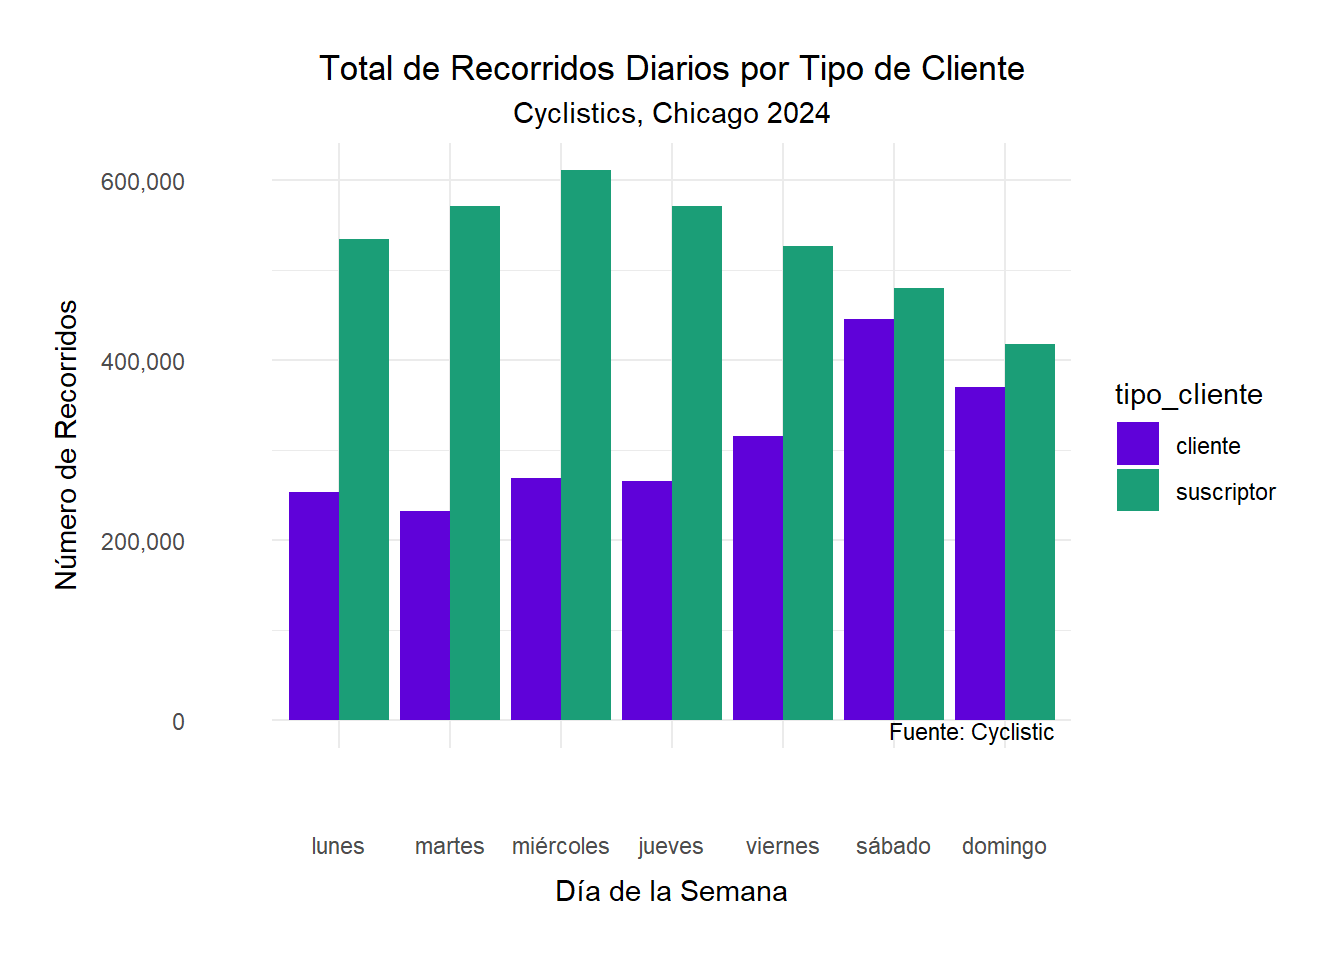
\includegraphics{Notebook_Cyclistics_files/figure-latex/unnamed-chunk-36-1.pdf}

\begin{enumerate}
\def\labelenumi{\arabic{enumi}.}
\setcounter{enumi}{2}
\tightlist
\item
  \textbf{Visualización:} '' Tiempo Medio Diario por Tipo de Cliente''
\end{enumerate}

\begin{Shaded}
\begin{Highlighting}[]
\CommentTok{\# Visualización: Tiempo promedio  de recorridos por tipo de cliente en dias de la semana}
\FunctionTok{ggplot}\NormalTok{(data\_resumen\_semana, }\FunctionTok{aes}\NormalTok{(}\AttributeTok{x =}\NormalTok{ dia\_semana, }\AttributeTok{y =}\NormalTok{ tiempo\_promedio, }\AttributeTok{fill =}\NormalTok{ tipo\_cliente)) }\SpecialCharTok{+}
  \FunctionTok{geom\_col}\NormalTok{(}\AttributeTok{position =} \StringTok{"dodge"}\NormalTok{) }\SpecialCharTok{+}
  \FunctionTok{scale\_fill\_manual}\NormalTok{(}\AttributeTok{values =}\NormalTok{ colores\_clientes) }\SpecialCharTok{+} \CommentTok{\# Aplicar la paleta de colores específica}
  \FunctionTok{scale\_y\_continuous}\NormalTok{(}\AttributeTok{labels =}\NormalTok{ comma) }\SpecialCharTok{+} \CommentTok{\# Cambia el formato del eje Y}
  \FunctionTok{labs}\NormalTok{(}
    \AttributeTok{title =} \StringTok{"Tiempo Promedio de Recorridos Durante la Semana por Tipo de Cliente"}\NormalTok{,}
    \AttributeTok{subtitle =} \StringTok{"Cyclistics, Chicago 2024"}\NormalTok{,}
    \AttributeTok{x =} \StringTok{"Día de la Semana"}\NormalTok{, }\AttributeTok{y =} \StringTok{"Tiempo Promedio (min)"}
\NormalTok{  ) }\SpecialCharTok{+}
  \FunctionTok{theme\_minimal}\NormalTok{() }\SpecialCharTok{+}
  \FunctionTok{theme}\NormalTok{( }
    \AttributeTok{plot.title =} \FunctionTok{element\_text}\NormalTok{(}\AttributeTok{hjust =} \FloatTok{0.5}\NormalTok{), }\CommentTok{\# Centra el título }
    \AttributeTok{plot.subtitle =} \FunctionTok{element\_text}\NormalTok{(}\AttributeTok{hjust =} \FloatTok{0.5}\NormalTok{), }\CommentTok{\# Centra el subtítulo}
    \AttributeTok{axis.text.x =} \FunctionTok{element\_text}\NormalTok{(}\AttributeTok{margin =} \FunctionTok{margin}\NormalTok{(}\AttributeTok{t =} \DecValTok{30}\NormalTok{, }\AttributeTok{b=}\DecValTok{5}\NormalTok{)), }\CommentTok{\# Añadir margen superior a las etiquetas del eje X }
    \AttributeTok{axis.text.y =} \FunctionTok{element\_text}\NormalTok{(}\AttributeTok{margin =} \FunctionTok{margin}\NormalTok{(}\AttributeTok{r =} \DecValTok{30}\NormalTok{, }\AttributeTok{l=}\DecValTok{5}\NormalTok{)), }\CommentTok{\# Añadir margen derecho a las etiquetas del eje Y}
\NormalTok{  ) }\SpecialCharTok{+}
  \FunctionTok{annotate}\NormalTok{(}\StringTok{"text"}\NormalTok{, }\AttributeTok{x =} \ConstantTok{Inf}\NormalTok{, }\AttributeTok{y =} \SpecialCharTok{{-}}\ConstantTok{Inf}\NormalTok{, }\AttributeTok{label =} \StringTok{"Fuente: Cyclistic"}\NormalTok{, }\AttributeTok{hjust =} \FloatTok{1.1}\NormalTok{, }\AttributeTok{vjust =} \SpecialCharTok{{-}}\FloatTok{0.5}\NormalTok{, }\AttributeTok{size =} \DecValTok{3}\NormalTok{)}
\end{Highlighting}
\end{Shaded}

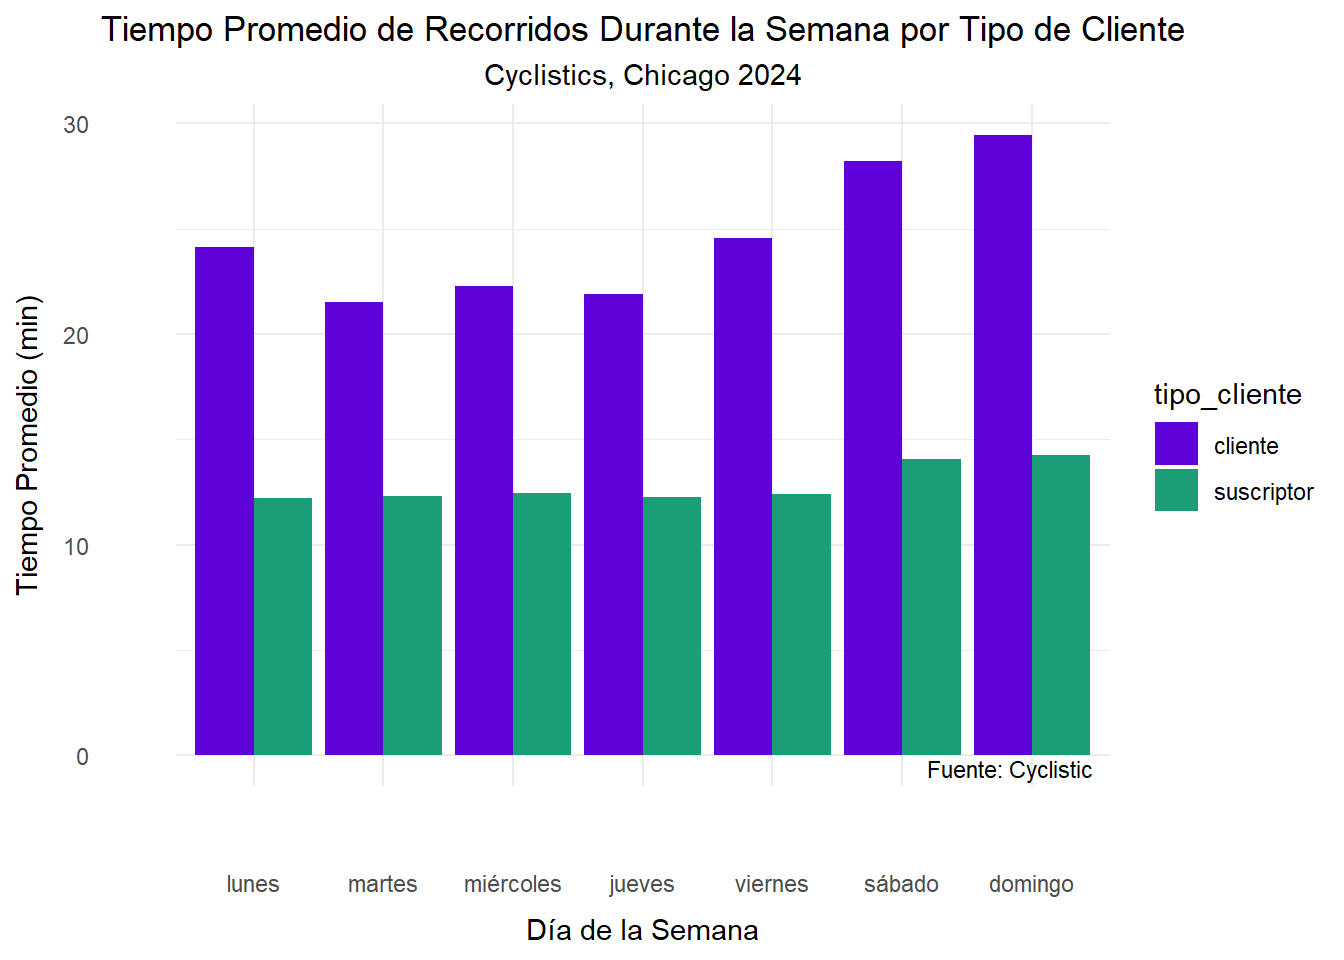
\includegraphics{Notebook_Cyclistics_files/figure-latex/unnamed-chunk-37-1.pdf}

\end{document}
